\documentclass{beamer}
\usepackage{graphicx}
\usepackage{tikz}
\usetikzlibrary{shapes,arrows}
\usepackage{tikz}
%\usecolortheme{seahorse}
  \setbeamertemplate{footline}[page number]
\usepackage{multirow}
\setbeamertemplate{navigation symbols}{}
\setbeamertemplate{frametitle}[default][center]
\setbeamerfont{frametitle}{shape=\scshape}
\usepackage{color}

\usepackage{csquotes}

\usepackage{xcolor}

\usepackage[flushleft]{threeparttable}

{\title{\textsc{Econ 352 - A Closed-Economy. One-Period Macroeconomic Model} \\ \tiny (See Williamson Ch. 5)}
\author{Trevor S. Gallen}
\date{}
\begin{document}
\renewcommand*{\inserttotalframenumber}{\pageref{lastframe}}


\setbeamertemplate{caption}{\raggedright\insertcaption\par}

\begin{frame}
\titlepage
\end{frame}

\begin{frame}
\frametitle[alignment=center]{Taking stock}
\begin{itemize}
\item We have a representative consumer/household that likes to consume and leisure, and works for wages, maximizing happiness
\bigskip
\item We have a representative firm that produces/sells good while maximizes profits by choosing labor
\bigskip
\item Now we put the together!
\end{itemize}
\end{frame}


\begin{frame}
\frametitle[alignment=center]{Some Terms and Assumptions}
\begin{itemize}
\item Right now we'll have a ``closed economy" which is a model of a single country with no interactions (no imports or exports:  everything that's produed will be consumed or invested)
\bigskip
\item This is different from an ``open economy" which is when international trade is allowed
\bigskip
\item The results for this chapter won't change much if we go to open economy, but the closed framework is useful for now
\bigskip
\item Adding in government:  for now, we're going to have an ``exogenous" amount of $G$ that is determined outside the model (not endogenous, determined within the model, like labor)
\item Government budget constraint will be simple:
$$G=T$$
\item This will allow for some basic analysis of \textbf{fiscal policy}, government spending
\end{itemize}
\end{frame}

\begin{frame}
\frametitle[alignment=center]{Competitive Equilibrium-Informal}
\begin{itemize}
\item Here we define a ``competitive equilibrium"
\bigskip
\item We have three exogenous variables:  $G$, $z$, $K$, which are exogenous, e.g. we take them as given
\bigskip
\item We want to solve for the endogenous variables: $C,N^s,N^d,T,Y$, and $w$
\bigskip
\item Our assumptions are that households and firms are maximizing, and that ``markets clear"
\bigskip
\item For instance, the labor market clears at a wage $w^*$ when, given that wage, the amount of labor households wish to supply is equal to the amount of labor firms demand.  
\end{itemize}
\end{frame}

\begin{frame}
\frametitle[alignment=center]{Competitive Equilibrium-Formal}
\begin{enumerate}
\item Representative consumer chooses $C$ (consumption) $N^s$ (labor supply) to maximize utility subject to $w$ (real wage) $T$ (taxes) and $\pi$ (dividend income
\item Representative firm chooses $N^d$ (quantity of labor demanded) to maximize profits, with output $Y=zF(K,N^d)$ and maximized profits $\pi=Y-wN^d$, taking $z$ and $K$ as given
\item Market for labor clears:  $N^d=N^s$
\item The government budget constraint is satisfied:  $G=T$
\end{enumerate}
\begin{itemize}
\item Usefully, all this implies $Y=C+G$, the income-expenditure identity
\end{itemize}
\end{frame}

\begin{frame}
\frametitle[alignment=center]{Competitive Equilibrium-Formal}
\begin{enumerate}
\item Representative consumer chooses $C$ (consumption) $N^s$ (labor supply) to maximize utility subject to $w$ (real wage) $T$ (taxes) and $\pi$ (dividend income
\item Representative firm chooses $N^d$ (quantity of labor demanded) to maximize profits, with output $Y=zF(K,N^d)$ and maximized profits $\pi=Y-wN^d$, taking $z$ and $K$ as given
\item Market for labor clears:  $N^d=N^s$
\item The government budget constraint is satisfied:  $G=T$
\end{enumerate}
\begin{itemize}
\item Usefully, all this implies $Y=C+G$, the income-expenditure identity
\end{itemize}
\end{frame}

\begin{frame}
\frametitle[alignment=center]{Finding our Equilibrium}
\begin{itemize}
\item Start with the production function:
$$Y=zF(K,N)$$
\item Then, use the fact that $N=N^s=N^d=h-\ell$
$$Y=zF(K,h-\ell)$$
\item Related to consumption via  feasibility :
$$C=zF(K,h-\ell)-G$$
\end{itemize}
\end{frame}

\begin{frame}
\frametitle[alignment=center]{Production Function and Production Possibilities Frontier}
\begin{figure}
\centering
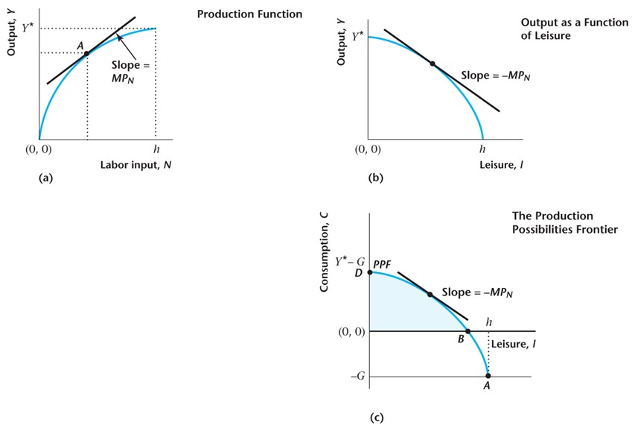
\includegraphics[scale=0.5]{Figures/W_Fig_5pt2.png}
\end{figure}
\end{frame}

\begin{frame}
\frametitle[alignment=center]{Putting Supply \& Demand Together}
\begin{itemize}
\item Recall from last class that the marginal rate of substitution of leisure for consumption for the household will be equal to the wage:
$$MRS_{\ell,C}=w$$
\item Also recall that the profit-maximizing amount of labor sets the marginal rate of transformation (the marginal product of labor) equal to the wage:
$$MP_N=w$$
\item This means that:
$$MRS_{\ell,C} =MRT_{\ell,C}=MP_N$$
\item It will turn out that this implies efficiency of the labor market, which we'll now discuss 
\end{itemize}
\end{frame}

\begin{frame}
\frametitle[alignment=center]{Production Function and Production Possibilities Frontier}
\begin{figure}
\centering
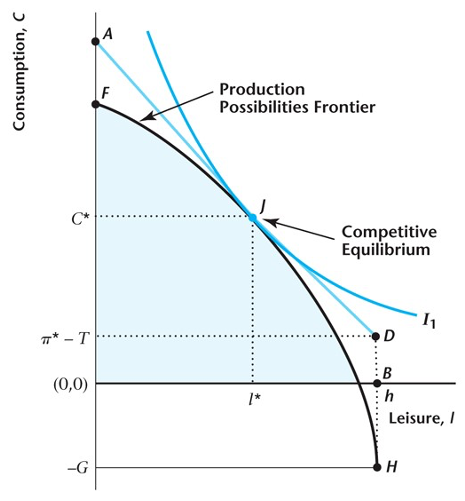
\includegraphics[scale=0.5]{Figures/W_Fig_5pt3.png}
\end{figure}
\end{frame}


\begin{frame}
\frametitle[alignment=center]{Efficiency}
\begin{itemize}
\item For economists, efficiency just means that people aren't ``unnecessarily" unhappy
\bigskip
\item Definition:  A competitive equilibrium is ``Pareto optimal" if there is no way to rearrange production or to reallocate goods so that someone is made better off without making someone else worse off
\bigskip
\item No transactions that would make both parties happier are left on the table
\bigskip
\item This will occur when the PPF, the frontier of possibilities, is tangent to preferences
\bigskip
\item If it weren't, then could improve! 
\end{itemize}
\end{frame}

\begin{frame}
\frametitle[alignment=center]{Production Function and Production Possibilities Frontier}
\begin{figure}
\centering
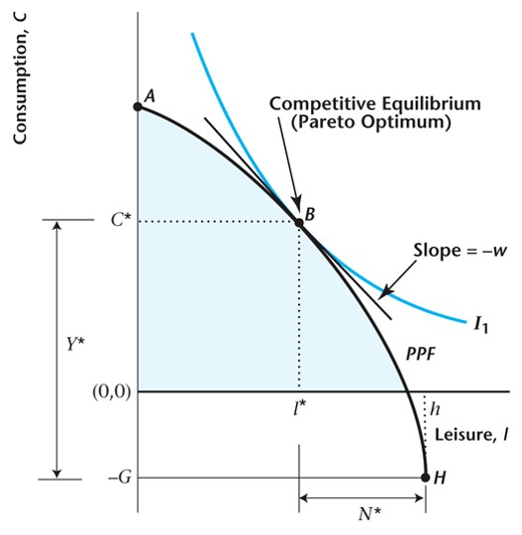
\includegraphics[scale=0.5]{Figures/W_Fig_5pt4.png}
\end{figure}
\end{frame}

\begin{frame}
\frametitle[alignment=center]{First Welfare Theorem}
\begin{itemize}
\item The \textbf{first fundamental  theorem of welfare economics} states that, under certain conditions, a competitive equilibrium is Pareto Optimal
\begin{itemize}
\item An old idea!  But leaves room for preferences
\end{itemize} 
\bigskip
\item The \textbf{second fundamental  theorem of welfare economics} states that, under certain conditions, a Pareto optimum is a competitive equilibrium
\begin{itemize}
\item You could achieve any Pareto optimum given starting conditions (free redistribution)
\end{itemize}
\item What breaks these?  The biggest is \textbf{externalities}
\end{itemize}
\end{frame}

\begin{frame}
\frametitle[alignment=center]{Sources of Social Inefficiencies-Externalities}
\begin{itemize}
\item Competitive equilibrium may not be Pareto optimal because of externalities 
\bigskip
\item If my private benefit for doing something is greater than the total public benefit (which includes my private) then I may do too much of it
\bigskip
\item For instance, let's say that I enjoy being warm, so I have preferences over log burning of:
$$U(burn)=\log(logs)-n$$
\item Where logs cost 1 work (so $logs=n$)
\bigskip
\item On my own, I maximize utility when $x=1$, which will set the PPF slope (1) equal my MRS (1/1=1).  
\bigskip
\item Efficient!  But if society doesn't like squared pollution, so that social costs are: $Scost=burn^2$, then while I would pick $1$, the socially optimal thing (including my own benefit and costs to others) would be to burn only 0.5 logs.  
\end{itemize}
\end{frame}

\begin{frame}
\frametitle[alignment=center]{Sources of Social Inefficiencies-Taxes}
\begin{itemize}
\item Competitive equilibrium may not be Pareto optimal because of distorting taxes 
\bigskip
\item I will set the marginal benefit of doing something equal to the \textbf{full} marginal cost (including taxes)
\bigskip
\item But that means that if taxes increase marginal cost, I will have to increase marginal benefit, which I can do (for things with diminishing utility) by reducing them
\bigskip
\item Let's take working for consumption, where I dislike working and like consumption:
$$U(C)=\sqrt{C}-n$$
\item Where my budget constraint is: $C=(1-\tau)n$ (wage is one)
\bigskip
\item Then, maximizing my utility, I get:
$$n=\frac{1-\tau}{4}\ \ \ C=\frac{(1-\tau)^2}{4}$$
\bigskip
\item For instance, if $\tau=0$, $C=n=0.25,U=-1.64$, $MRS_{\ell,c}=2\sqrt{C}=1=w=MP_n$
\item If $\tau=0.5$, $C=0.0625$, $n=0.125$, $U=-2.90$ $MRS_{\ell,c}=0.5=(1-\tau)w<w=MP_n$
\item There's a ``wedge" between MRS and $MP_n$ (of $\tau$)
\end{itemize}
\end{frame}


\begin{frame}
\frametitle[alignment=center]{Sources of Social Inefficiencies-Taxes Example}
\begin{itemize}
\item Let's take working for consumption, where I dislike working and like consumption:
$$U(C)=\sqrt{C}-n$$
\item Where my budget constraint is: $C=(1-\tau)n$ (wage is one)
\bigskip
\item Then, maximizing my utility, I get:
$$n=\frac{1-\tau}{4}\ \ \ C=\frac{(1-\tau)^2}{4}$$
\bigskip
\item For instance, if $\tau=0$, $C=n=0.25,U=-1.64$, $MRS_{\ell,c}=2\sqrt{C}=1=w=MP_n$
\bigskip
\item If $\tau=0.5$, $C=0.0625$, $n=0.125$, $U=-2.90$ $MRS_{\ell,c}=0.5=(1-\tau)w<w=MP_n$
\bigskip
\item There's a ``wedge" between MRS and $MP_n$ (of $\tau$)
\end{itemize}
\end{frame}


\begin{frame}
\frametitle[alignment=center]{Sources of Social Inefficiencies-Firms are not Price Takers}
\begin{itemize}
\item If firms have monopoly power, or if unions/workers have monopsony power, then inefficiency can result
\bigskip
\item In both, there is another ``wedge."  Rather than the government artificially raising the cost of a good via a tax, a firm might artificially raise the cost of a good by restricting supply
\bigskip
\item Similarly, rather than a government increasing the cost of labor to firms via a tax, a union might do it via negotiation
\bigskip
\item In both, private benefit may mean leaving good (Pareto-improving) trades on the table
\end{itemize}
\end{frame}

\begin{frame}
\frametitle[alignment=center]{Production Function and Production Possibilities Frontier}
\begin{figure}
\centering
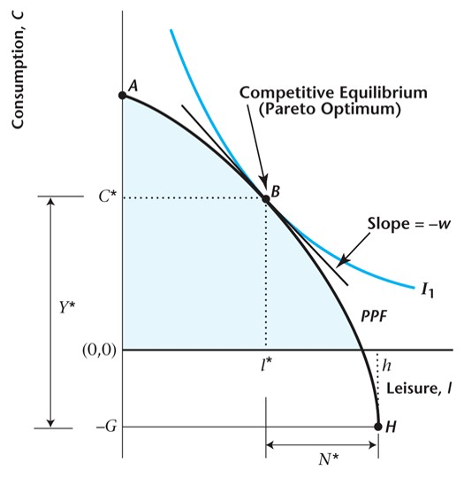
\includegraphics[scale=0.5]{Figures/W_Fig_5pt5.png}
\end{figure}
\end{frame}


\begin{frame}
\frametitle[alignment=center]{Applying the model:  changes in government purchases}
\begin{itemize}
\item Now we're going to apply our model in a very simple way:  we're going to have $G$ increase and ask what this does to $Y$, $C$, $n$, and $w$.
\bigskip
\item What happens?  Recall that $G=T$, so $\Delta G=\Delta T$, a shift out of government spending will be a shift out of taxes and a shift in of the PPF
\bigskip
\item We're poorer! So, consume less of all normal goods (less consumption, less leisure (more work)).  $\Delta C<0$, $\Delta n>0$. 
\bigskip
\item If $\Delta n >0$, and we know $w=MP_n=\frac{\partial zf(K,n)}{\partial n}$, and $\frac{\partial^2 zf(K,n)}{\partial n^2}<0$, $w$ falls (but by less than $n$ increases, from CRS)
\bigskip
\item From the budget constraint: if we're working more, then $-\Delta C<\Delta T$, and because $Y=C+G=C+T$, it must be that $\Delta Y>0$.  
\bigskip
\item I know this might be confusing, so let's see it graphically, then go through a concrete example!
\end{itemize}
\end{frame}

\begin{frame}
\frametitle[alignment=center]{Equilibrium Effects of an Increase in Government Spending}
\begin{figure}
\centering
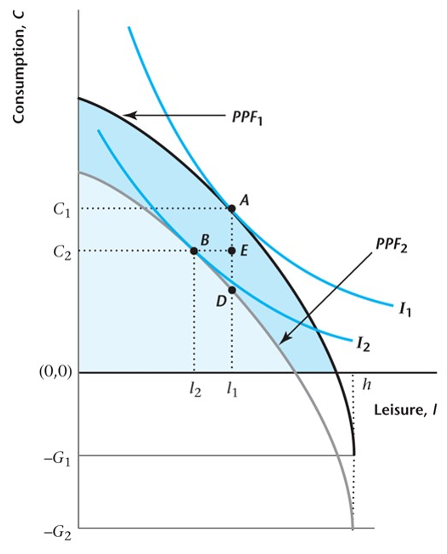
\includegraphics[scale=0.5]{Figures/W_Fig_5pt6.png}
\end{figure}
\end{frame}

\begin{frame}
\frametitle[alignment=center]{Concrete Example}
\begin{itemize}
\item Production function:  $Y=zn^{\alpha}$
\bigskip
\item Preferences+time budget constraint  $n=1-\ell$:  
$$U(C,n)=\sqrt{C}+\sqrt{1-n}$$
\item Budget constraint:  $C=nw+\pi-T$
\bigskip
\item Profit:  $\pi=Y-nw$
\bigskip
\item Government b.c. : $G=T$
\bigskip
\item We have 3 exogenous variables: $z$, $\alpha$, $G$
\bigskip
\item If we plug in the budget constraint into preferences to get rid of $C$, we have 7 endogenous variables: $Y$, $n$, $\ell$, $T$, $\pi$, $w$
\bigskip
\item And 7 equations:  (1) firm FOC wrt $n$ (``labor demand") (2) production function (``consumption supply"), (3) HH foc wrt $n$ (``labor supply"), (4) time budget constraint (5) HH budget constraint (``consumption demand") (6) government budget constraint and (7) profit condition
\end{itemize}
\end{frame}

\begin{frame}
\frametitle[alignment=center]{Seven Equations, Seven Unknowns}
\begin{table}
\begin{tabular}{ll}
\multicolumn{2}{c}{Seven Equations, Seven Unknowns}\\
\hline\hline
Firm FOC wrt $n$ & $\alpha zn^{\alpha-1}=w$ \\
Production function & $Y=zn^{\alpha}$\\
 HH foc wrt $n$:  & $n=\frac{w^2+T-\pi}{w(1+w)}$\\
 Time budget constraint & $n=1-\ell$\\
 Government budget constraint & $G=T$\\
 Profit definition & $\pi=Y-nw$\\
  HH Budget constraint & $C=nw+\pi-T$\\
  \hline
\end{tabular}
\end{table}
\begin{itemize}
\item While we could solve for this ``closed form" that's not what modern macroeconomists do 
\bigskip
\item Algebra is for suckers(?!)
\bigskip
\item Instead we hand off to solvers...let's look at excel!
\end{itemize}
\end{frame}


\begin{frame}
\frametitle[alignment=center]{Excel}
\begin{itemize}
\item See SimpleMacro.xlsx
\begin{table}
\begin{tabular}{lccc}
\multicolumn{4}{c}{Effects of an Increase in $G$}\\
\hline\hline
Variable & Baseline & G$\uparrow$33\% & \% Change\\
\hline
z & 1 & 1 & 0.00\%\\
$\alpha$ & 0.7 & 0.7 & 0.00\%\\
g & 0.3 & 0.4 & 33.33\%\\
n & 0.53 & 0.58 & 10.12\%\\
w & 0.85 & 0.82 & -2.85\%\\
Y & 0.64 & 0.68 & 6.98\%\\
$\ell$ & 0.47 & 0.42 & -11.32\%\\
$\pi$ & 0.19 & 0.21 & 6.98\%\\
T & 0.30 & 0.40 & 33.33\%\\
C & 0.34 & 0.28 & -16.31\%\\
\hline\hline
\end{tabular}
\end{table}
\end{itemize}
\end{frame}


\begin{frame}
\frametitle[alignment=center]{Summarizing the Simple Model}
\begin{itemize}
\item Simple excel model hopefully useful in a few ways
\bigskip
\item Never simplify again!  Just throw all your equations and solve numerically 
\bigskip
\item Confirms Williamson/our intuitive explanation of what should happen
\bigskip
\item Modern macro isn't so far from this...just make this an infinite period model/capital and you have Modern macro representative agent models: change G, how do things change?
\bigskip
\item Now let's move on to changes in total factor productivity ($z$), rather than changes in $G$
\end{itemize}
\end{frame}

\begin{frame}
\frametitle[alignment=center]{Shift in total factor productivity}
\begin{itemize}
\item Must break up into short and long-run.
\bigskip
\item Let's think about short run for now.
\bigskip
\item When $z$ increases, the PPF increases \emph{and} slope changes (income and substitution effects)
\bigskip
\item We know that $C$ will increase, but $n$ may rise or fall
\bigskip
\item $Y=C+G$, $G$ constant, so $Y$ increases (could also see from $n$ increasing)
\bigskip
\item If labor stayed the same, then $w$ increases ($MP_n\uparrow$) 
\bigskip
\item Let's see this graphically
\end{itemize}
\end{frame}

\begin{frame}
\frametitle[alignment=center]{Production Function and Production Possibilities Frontier}
\begin{figure}
\centering
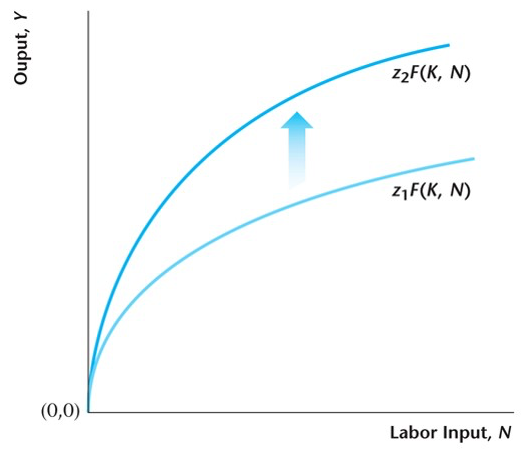
\includegraphics[scale=0.5]{Figures/W_Fig_5pt8.png}
\end{figure}
\end{frame}

\begin{frame}
\frametitle[alignment=center]{Competitive Equilibrium Effects of an Increase in TFP}
\begin{figure}
\centering
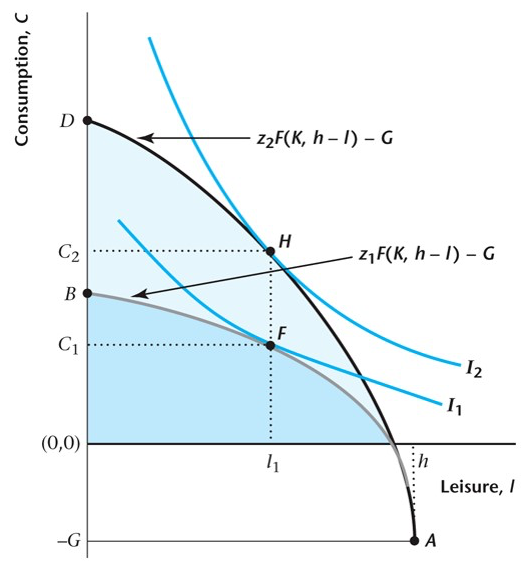
\includegraphics[scale=0.5]{Figures/W_Fig_5pt9.png}
\end{figure}
\end{frame}


\begin{frame}
\frametitle[alignment=center]{Income and Substitution Effects of an Increase in TFP}
\begin{figure}
\centering
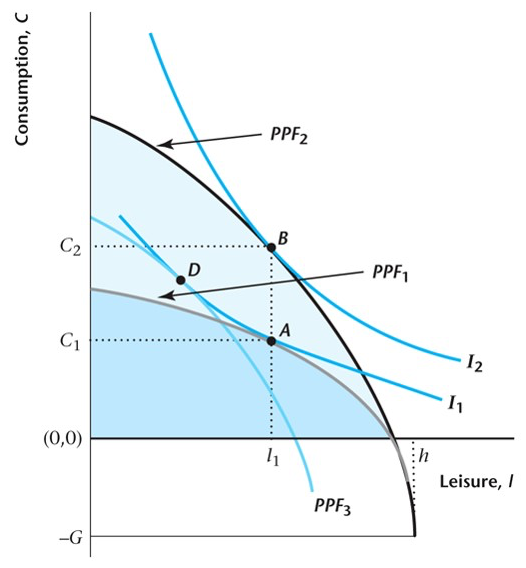
\includegraphics[scale=0.5]{Figures/W_Fig_5pt10.png}
\end{figure}
\end{frame}


\begin{frame}
\frametitle[alignment=center]{Another Concrete Example}
\begin{itemize}
\item Let's go through the same example, but now $z$ will increase rather than $G$
\item Production function:  $Y=zn^{\alpha}$
\bigskip
\item Preferences+time budget constraint  $n=1-\ell$:  
$$U(C,n)=\sqrt{C}+\sqrt{1-n}$$
\item Budget constraint:  $C=nw+\pi-T$
\bigskip
\item Profit:  $\pi=Y-nw$
\bigskip
\item Government b.c. : $G=T$
\bigskip
\item We have 3 exogenous variables: $z$, $\alpha$, $G$
\bigskip
\item If we plug in the budget constraint into preferences to get rid of $C$, we have 7 endogenous variables: $Y$, $n$, $\ell$, $T$, $\pi$, $w$
\bigskip
\item And 7 equations:  (1) firm FOC wrt $n$ (``labor demand") (2) production function (``consumption supply"), (3) HH foc wrt $n$ (``labor supply"), (4) time budget constraint (5) HH budget constraint (``consumption demand") (6) government budget constraint and (7) profit condition
\end{itemize}
\end{frame}

\begin{frame}
\frametitle[alignment=center]{Excel}
\begin{itemize}
\item See SimpleMacro.xlsx
\begin{table}
\begin{tabular}{lccc}
\multicolumn{4}{c}{Effects of an Increase in $z$}\\
\hline\hline
Variable & Baseline & z$\uparrow$5\% & \% Change\\
\hline
z & 1 & 1.05 & 5.00\%\\
$\alpha$ & 0.7 & 0.7 & 0.00\%\\
g & 0.3 & 0.3 & 0.00\%\\
n & 0.53 & 0.53 & 0.25\%\\
w & 0.85 & 0.89 & 4.92\%\\
Y & 0.64 & 0.67 & 5.19\%\\
$\ell$ & 0.47 & 0.47 & -0.28\%\\
$\pi$ & 0.19 & 0.20 & 5.19\%\\
T & 0.30 & 0.30 & 0.00\%\\
C & 0.34 & 0.37 & 9.77\%\\
\hline\hline
\end{tabular}
\end{table}
\end{itemize}
\end{frame}


\begin{frame}
\frametitle[alignment=center]{Takeaways}
\begin{itemize}
\item What can we do with this simple model?
\bigskip
\item Since WWII, $z$ has increased dramatically, while $Y$, $w$, $C$, have gone up, and $n$ has remained roughly constant
\bigskip
\item Our simple prediction is that when $z$ increases, $Y$, $w$, $C$, will go up, and we've noted an ambiguity in $n$ (for our specific calibration, it increased)
\bigskip
\item Idea:  if we had preferences where income and substitution effects that cancel (so $w\uparrow$, $n\cdot$, then our model would be consistent
\bigskip
\item But our model helps give an idea about short- and long-run.  We saw that in the short run, $L$ moves with $w$, so short run substitution effect should dominate, but long run should cancel.
\bigskip
\item As we'll discuss, this would make sense if temporary shocks didn't increase \emph{lifetime} income much, but did increase wages
\bigskip
\item This leads to the debate over \textbf{real business cycle theory}, and whether the \textbf{intertemporal substitution of labor} is a big enough factor to explain labor over the business cycle
\end{itemize}
\end{frame}

\begin{frame}
\frametitle[alignment=center]{Let's look at some data}
\begin{itemize}
\item First we'll look at TFP \& GDP, then at
\bigskip
\item Since WWII, $z$ has increased dramatically, while $Y$, $w$, $C$, have gone up, and $n$ has remained roughly constant
\bigskip
\item Our simple prediction is that when $z$ increases, $Y$, $w$, $C$, will go up, and we've noted an ambiguity in $n$ (for our specific calibration, it increased)
\bigskip
\item Idea:  if we had preferences where income and substitution effects that cancel (so $w\uparrow$, $n\cdot$, then our model would be consistent
\bigskip
\item But our model helps give an idea about short- and long-run.  We saw that in the short run, $L$ moves with $w$, so short run substitution effect should dominate, but long run should cancel.
\bigskip
\item As we'll discuss, this would make sense if temporary shocks didn't increase \emph{lifetime} income much, but did increase wages
\bigskip
\item This leads to the debate over \textbf{real business cycle theory}, and whether the \textbf{intertemporal substitution of labor} is a big enough factor to explain labor over the business cycle
\end{itemize}
\end{frame}


\begin{frame}
\frametitle[alignment=center]{TFP and GDP over the Business Cycle}
\begin{figure}
\centering
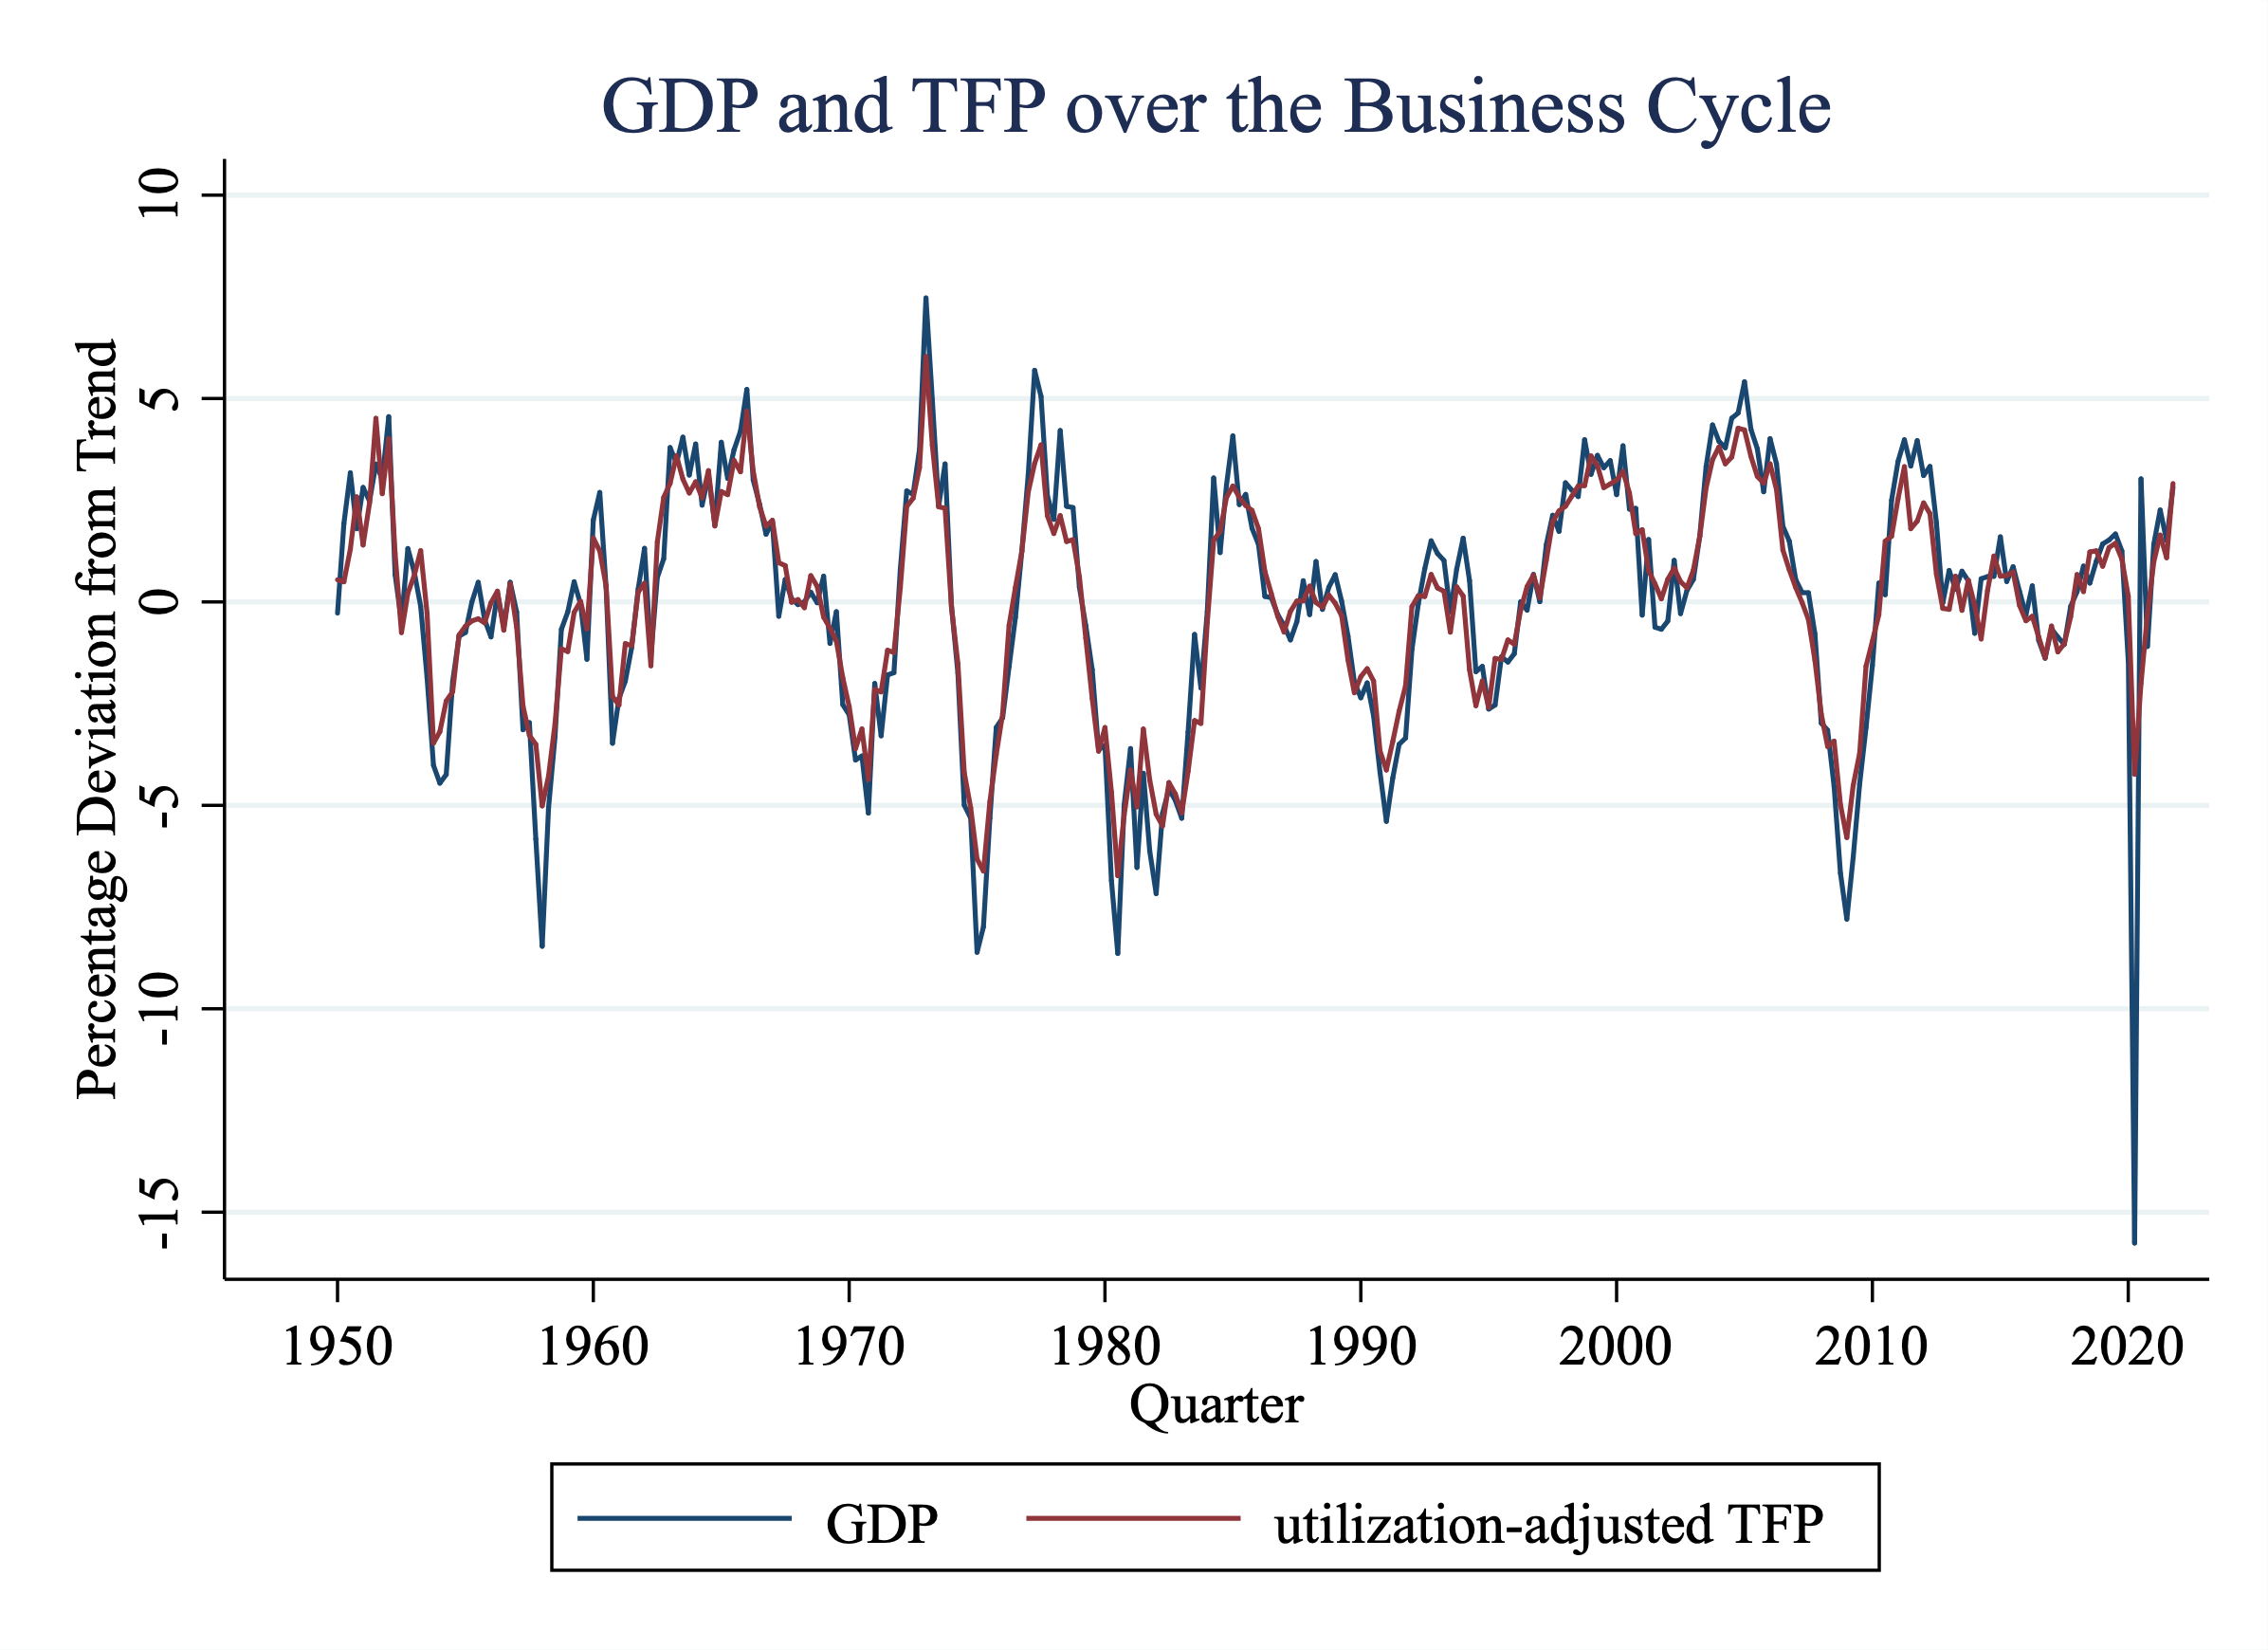
\includegraphics[scale=0.2]{Figures/GDP_TFP_buscycle.png}
\end{figure}
TFP and GDP move together--it explains growth, what about the business cycle?  
\end{frame}

\begin{frame}
\frametitle[alignment=center]{Let's look at some more data}
\begin{itemize}
\item Now let's look at what's happened to government spending over time, to link back to our discussion of government purchases
\end{itemize}
\end{frame}




\begin{frame}
\frametitle[alignment=center]{Y, C, and G over time}
\begin{figure}
\centering
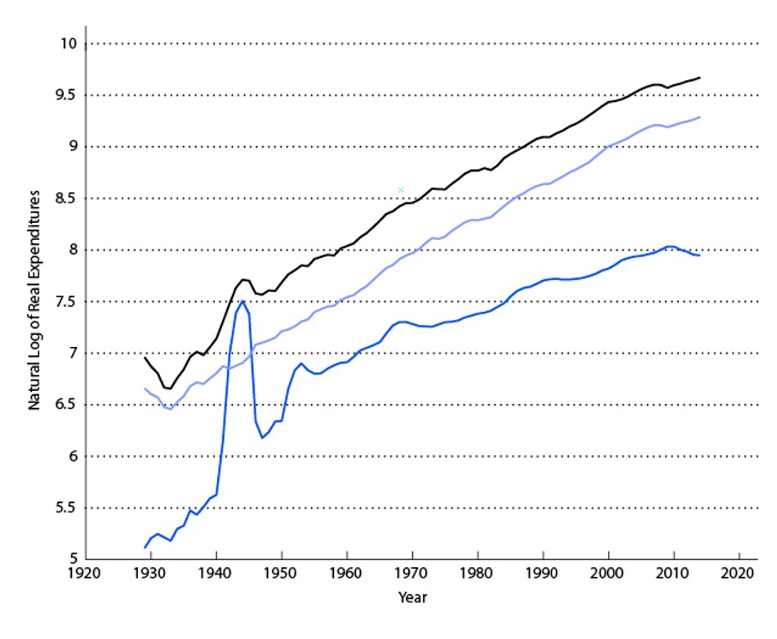
\includegraphics[scale=0.5]{Figures/W_Fig_5pt7.png}
\end{figure}
What about Covid times?
\end{frame}

\begin{frame}
\frametitle[alignment=center]{Y, C, and G over time-updated}
\begin{figure}
\centering
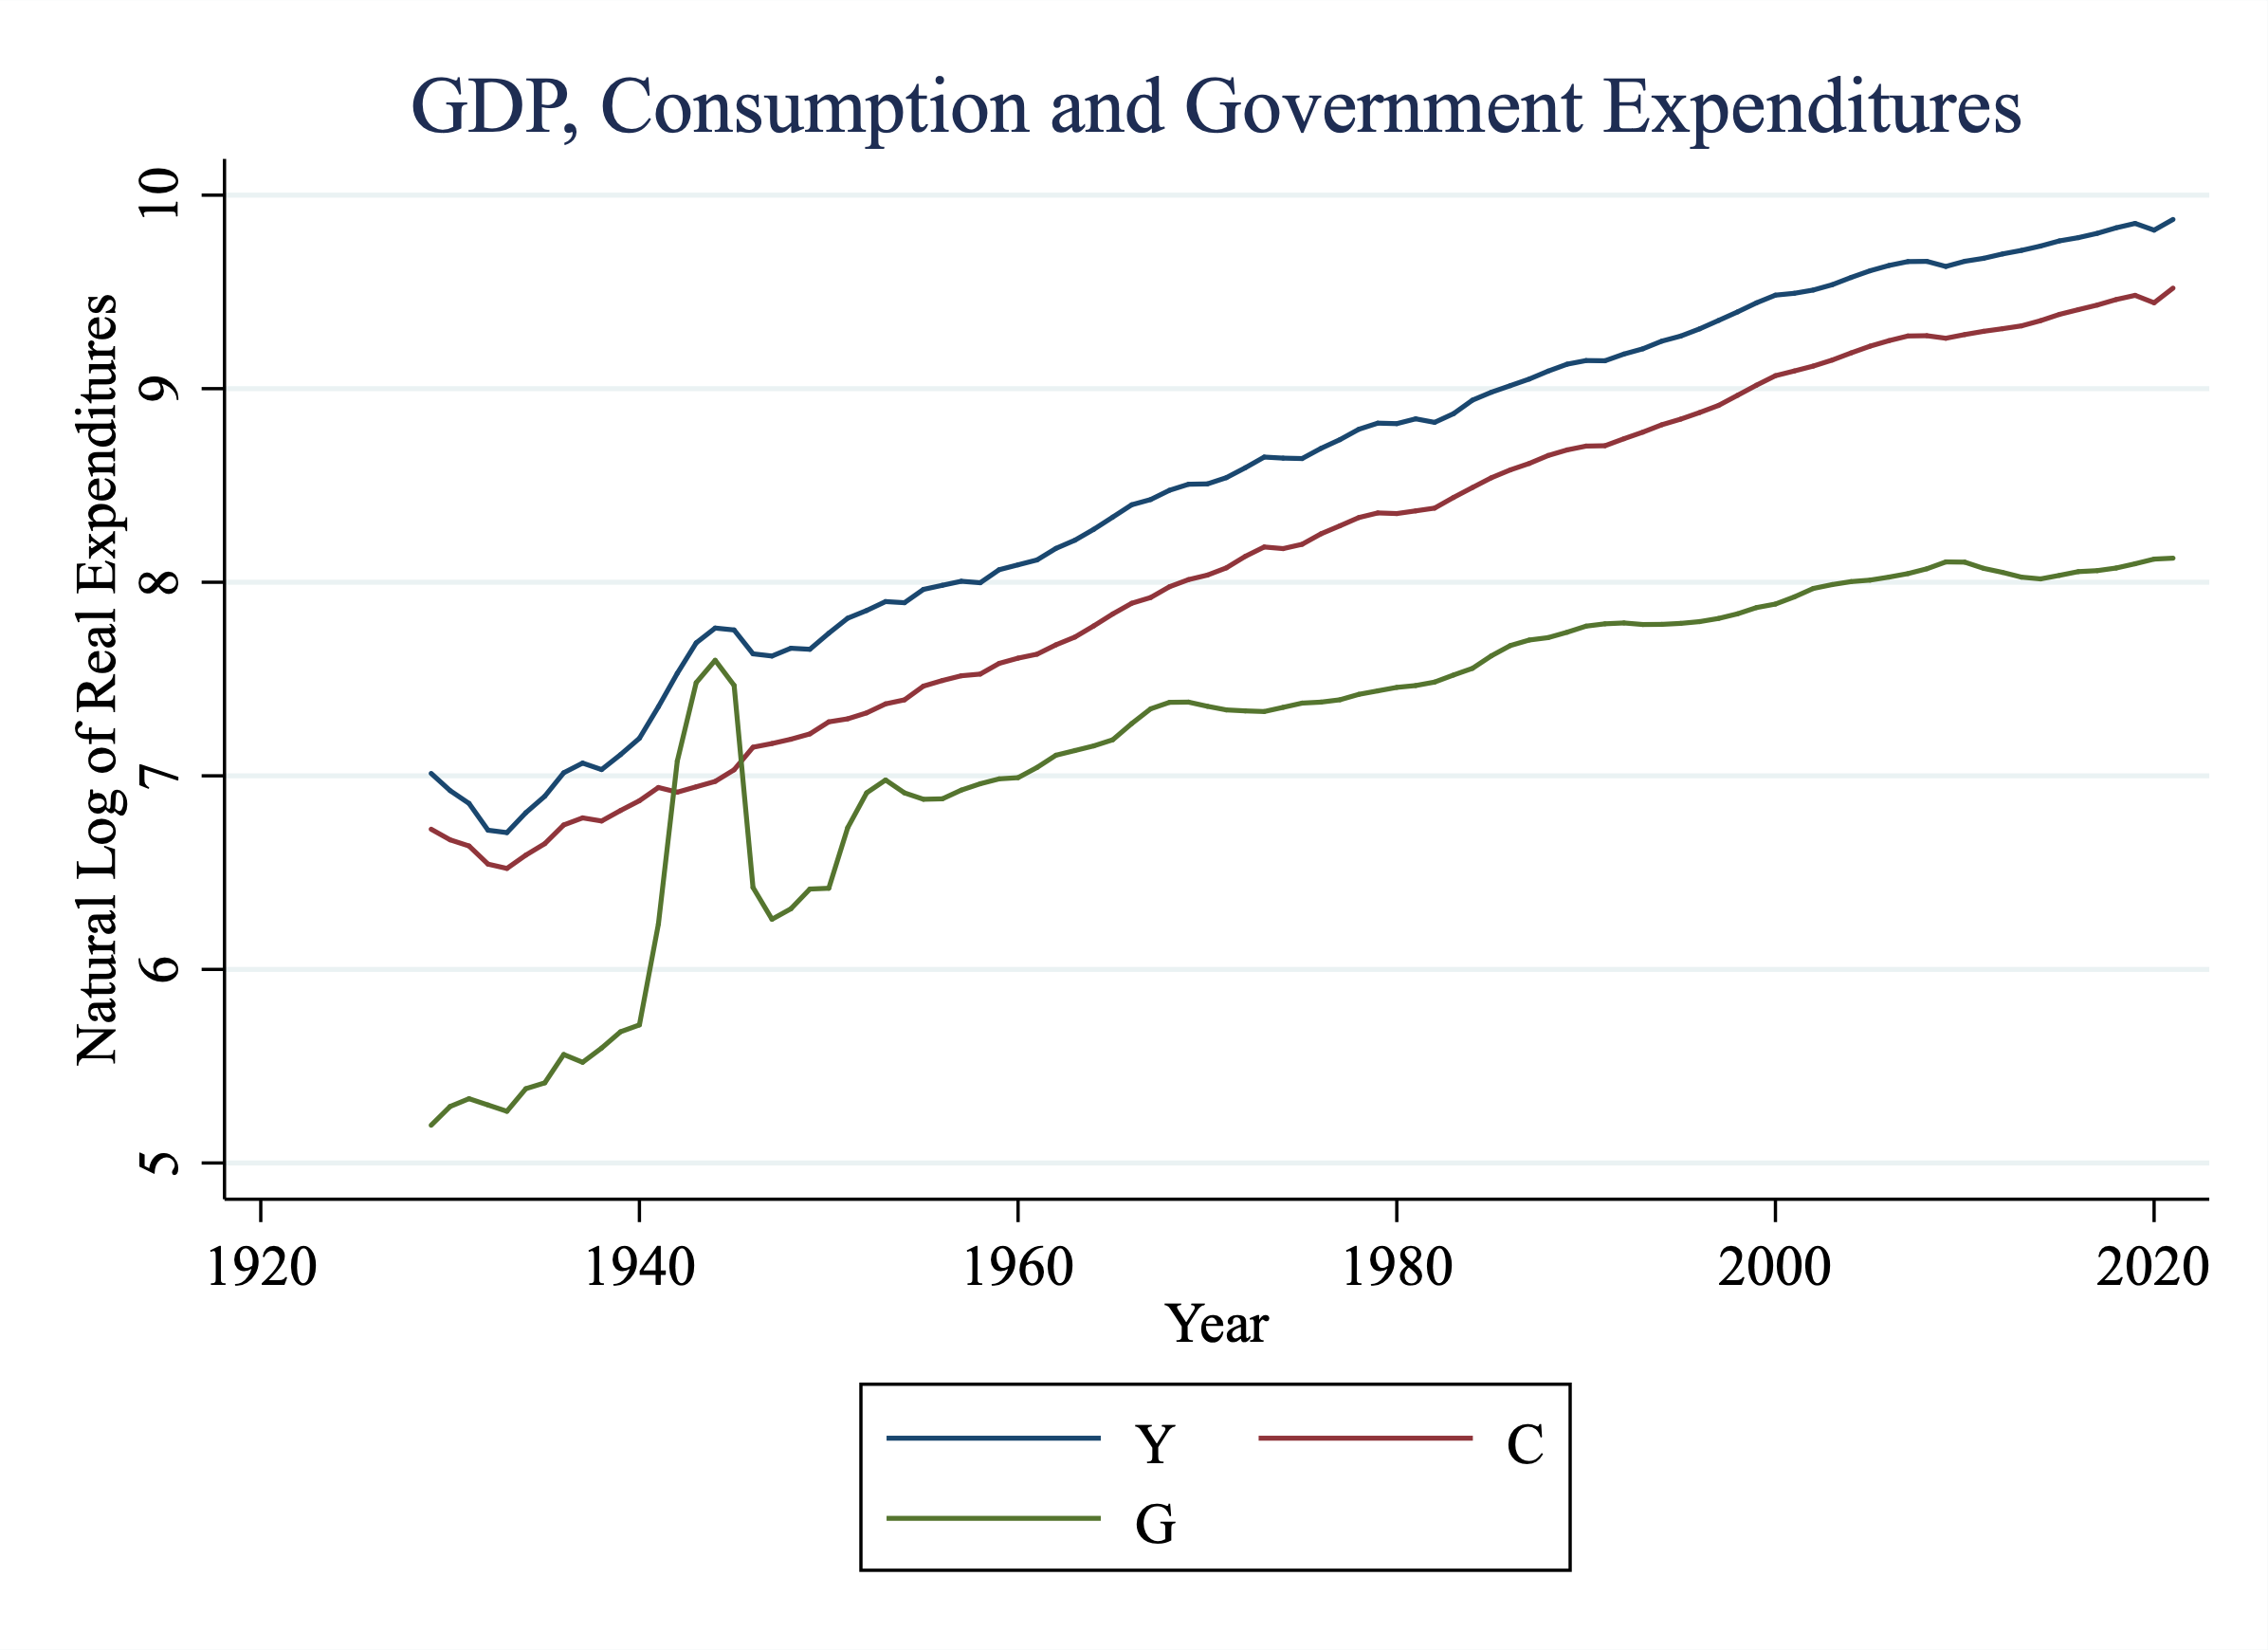
\includegraphics[scale=0.2]{Figures/Y_C_G.png}
\end{figure}
\end{frame}

\begin{frame}
\frametitle[alignment=center]{Government expenditures over time}
\begin{figure}
\centering
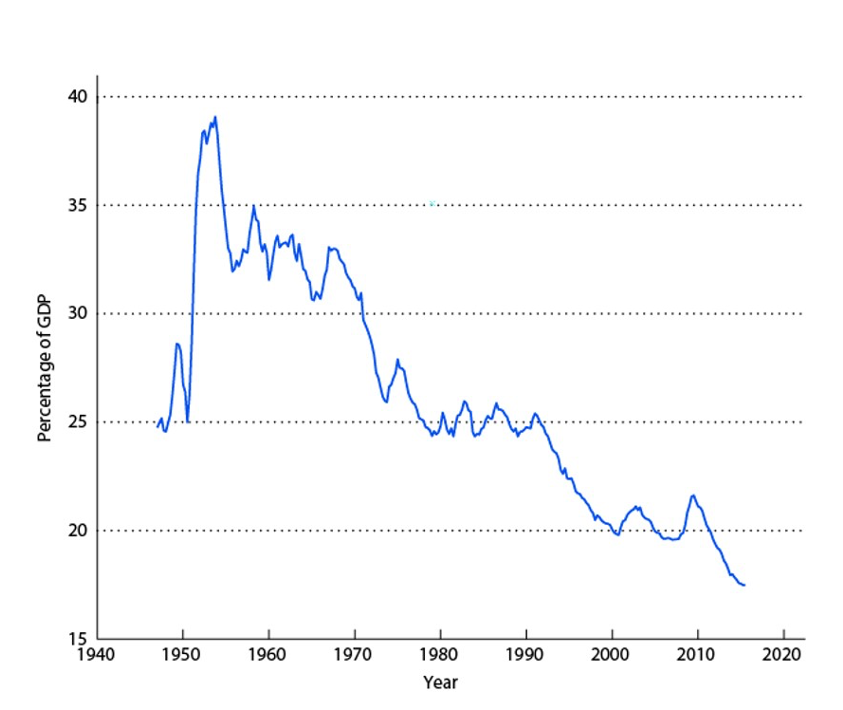
\includegraphics[scale=0.5]{Figures/W_Fig_5pt12.png}
\end{figure}
Is government declining as a fraction of GDP?
\end{frame}

\begin{frame}
\frametitle[alignment=center]{Government expenditures over time-updated}
\begin{figure}
\centering
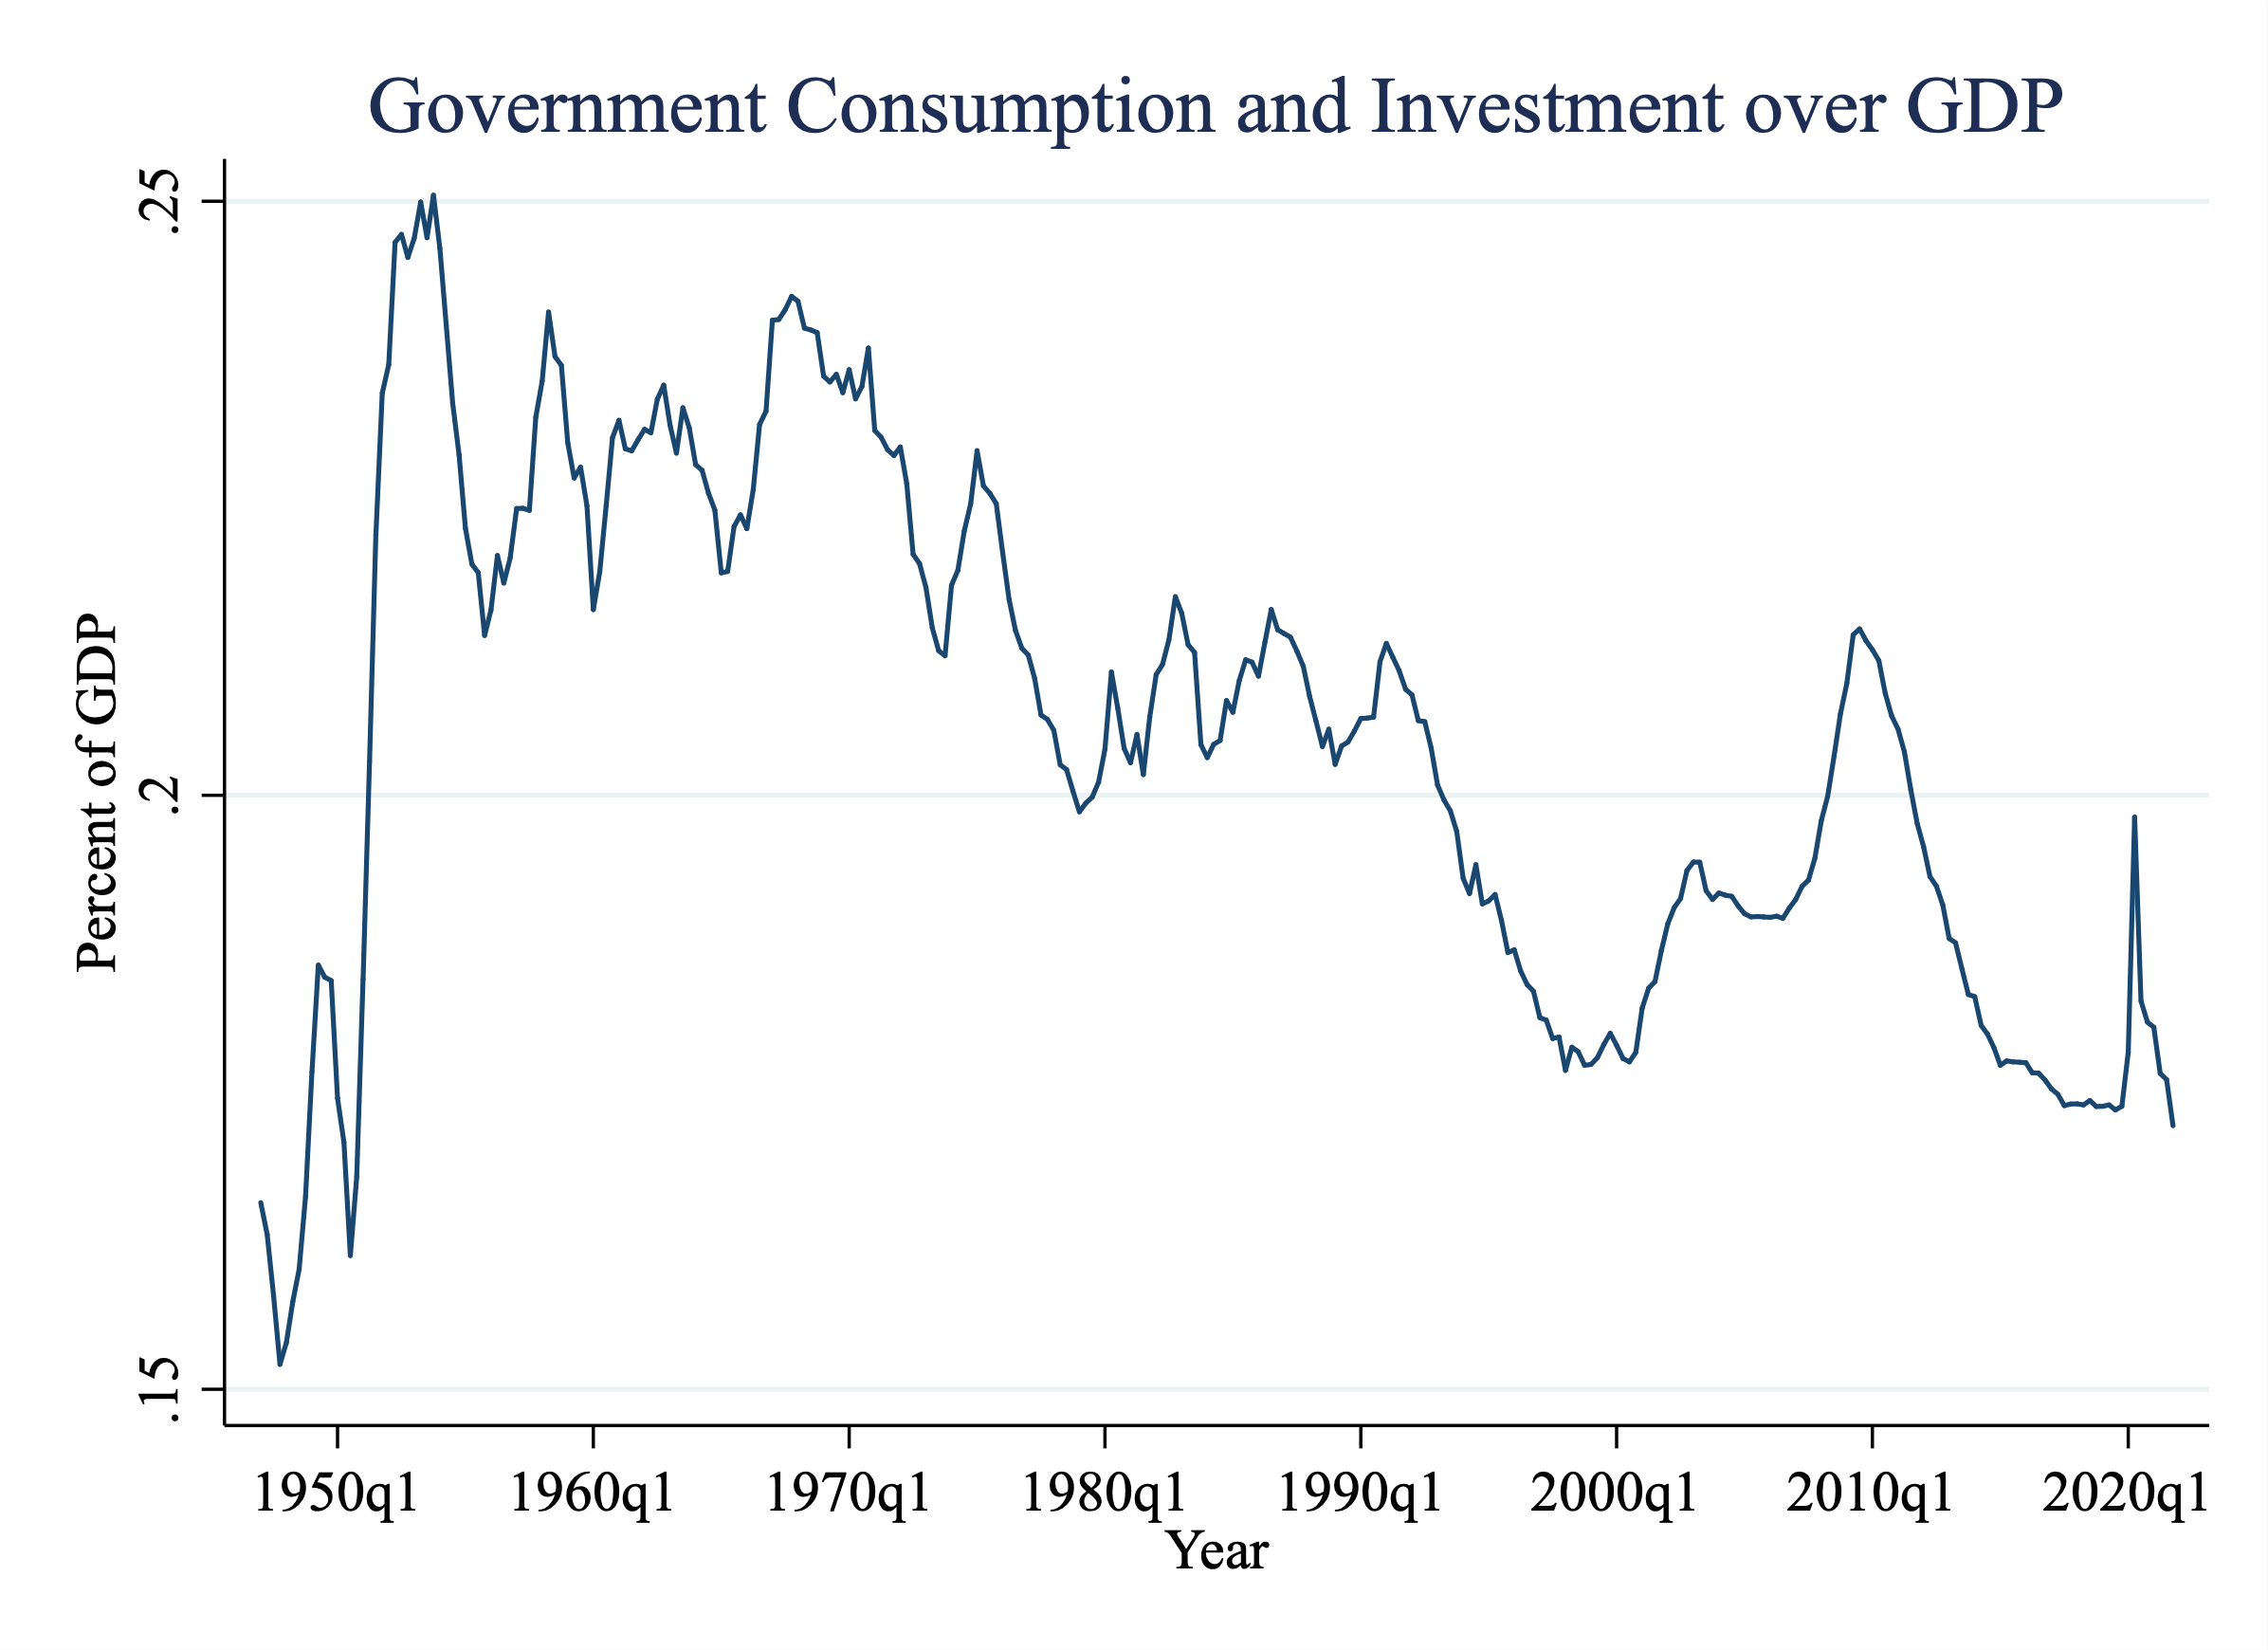
\includegraphics[scale=0.2]{Figures/GoverY_1.png}
\end{figure}
\end{frame}

\begin{frame}
\frametitle[alignment=center]{Government outlays over time-updated}
\begin{figure}
\centering
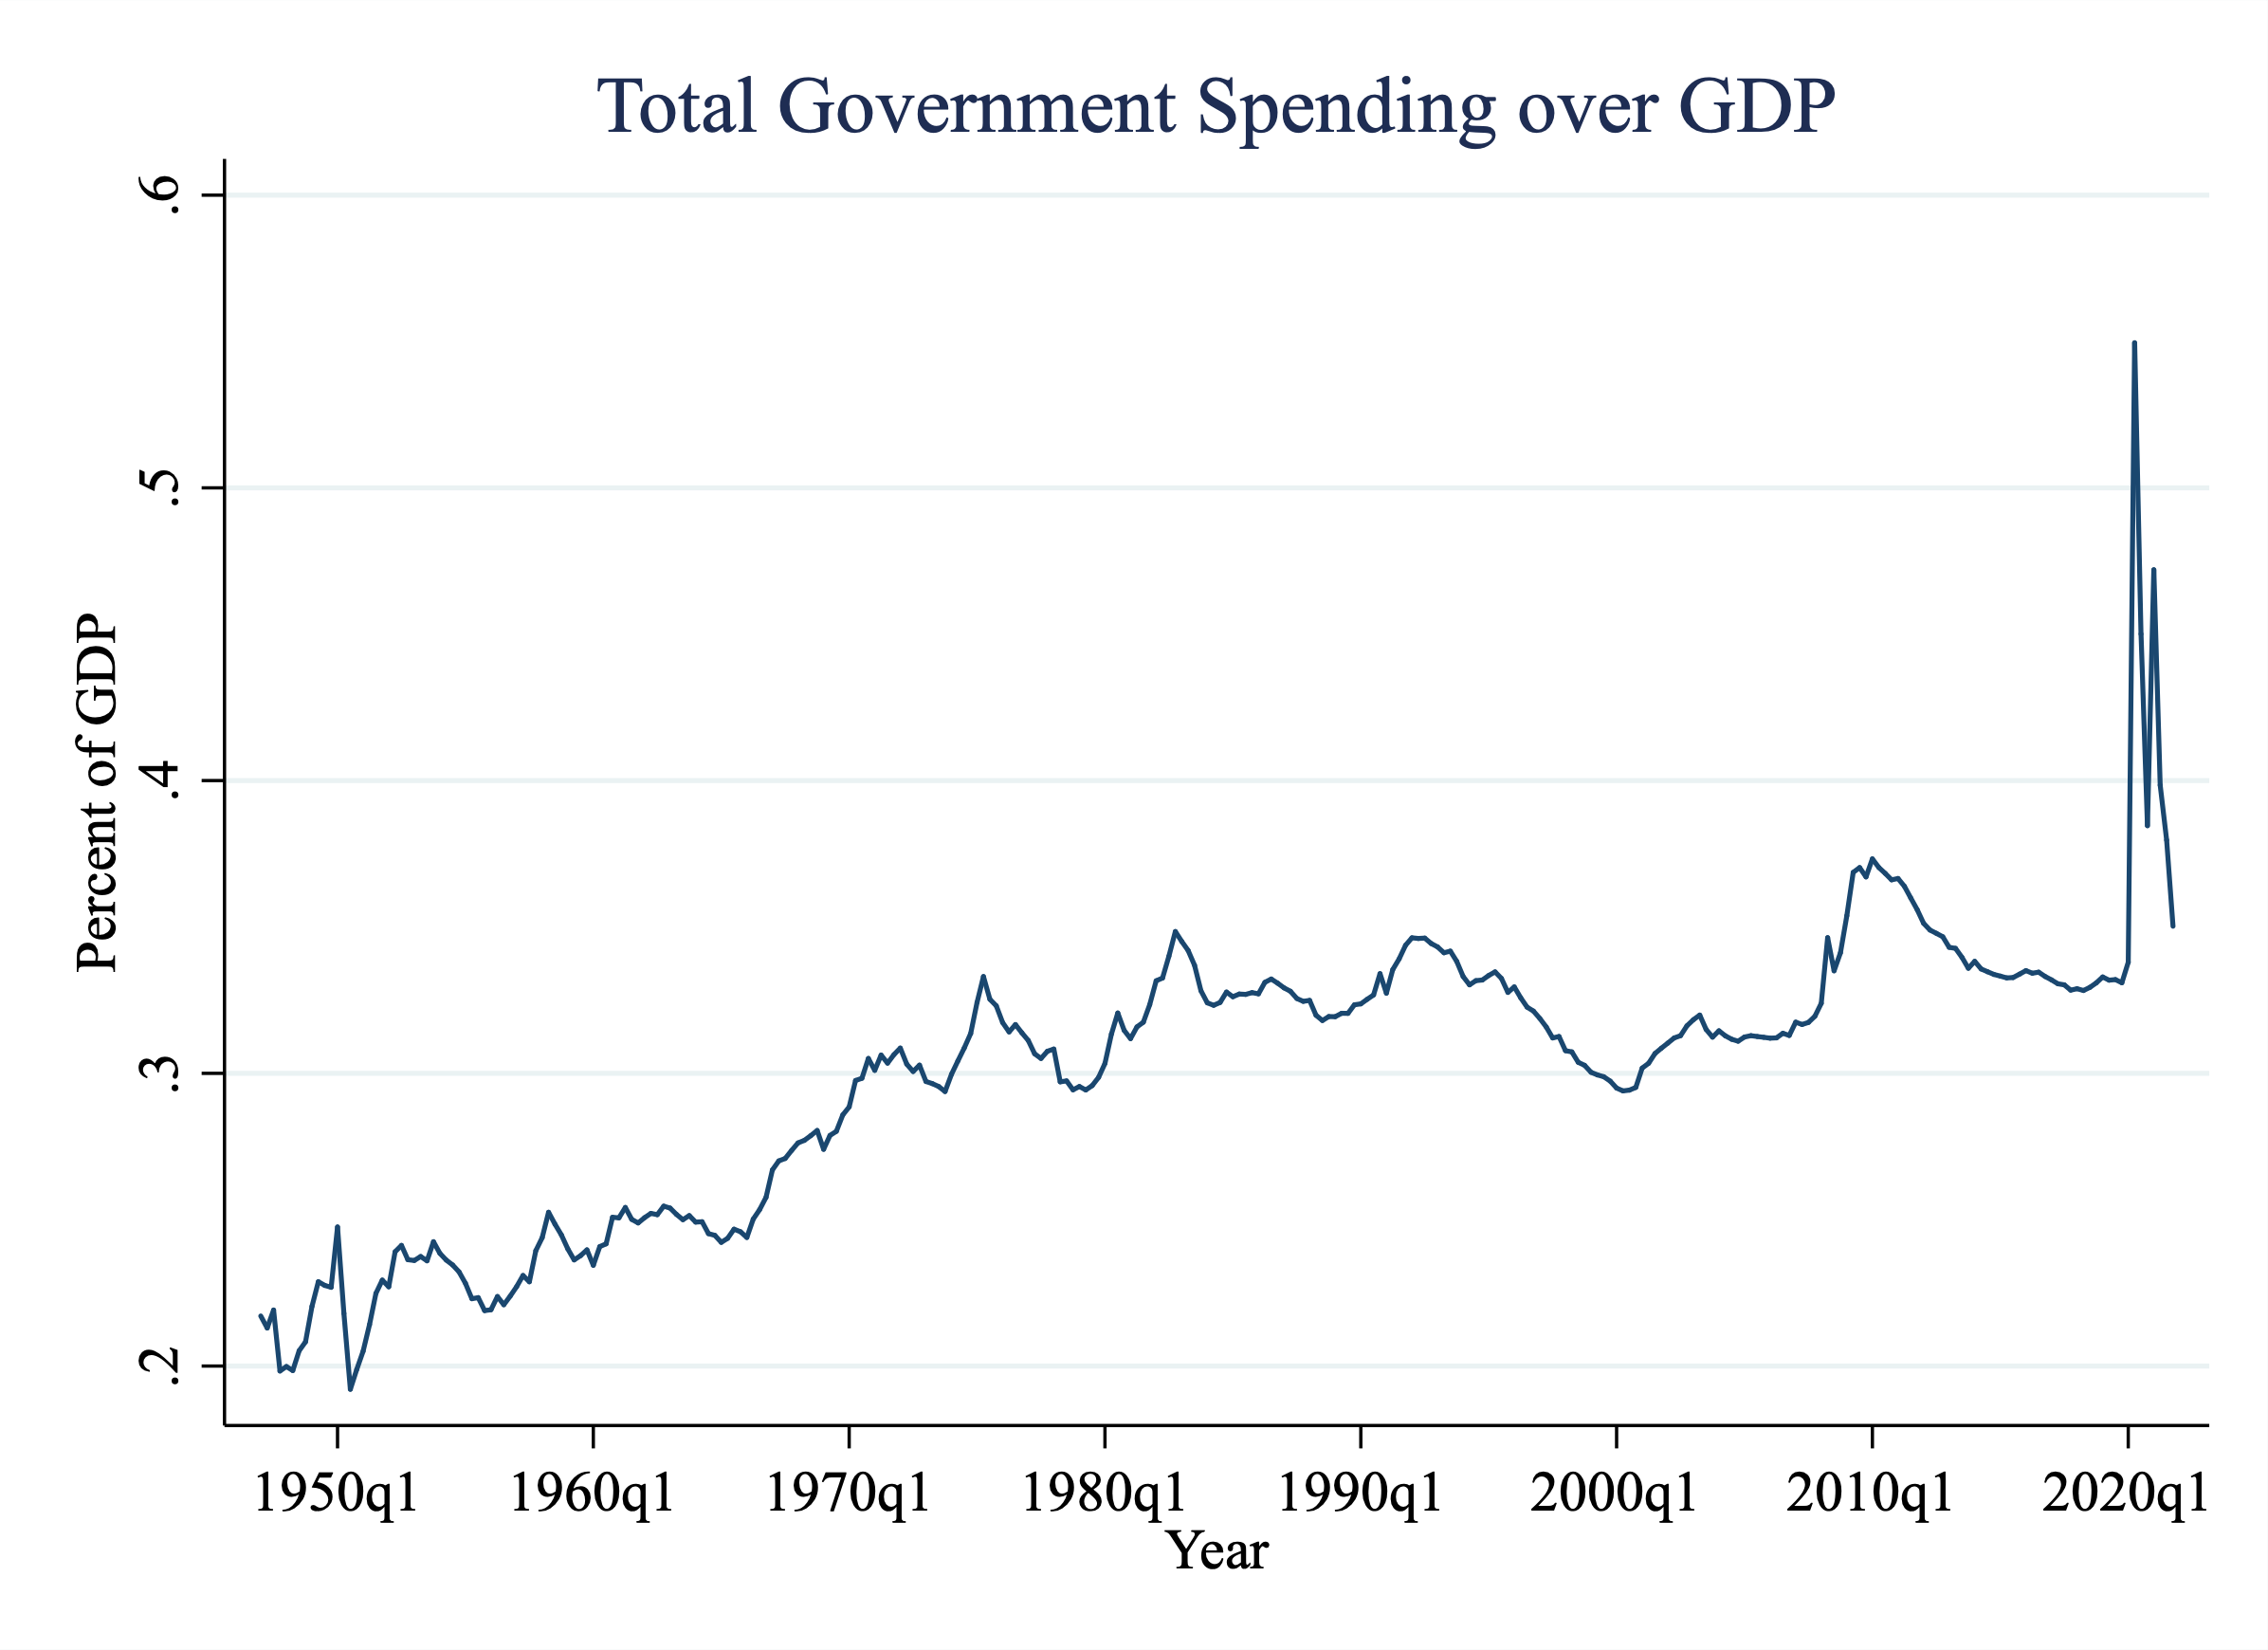
\includegraphics[scale=0.2]{Figures/GoverY_2.png}
\end{figure}
No!  It's...expanding? (also...Covid!!)
\end{frame}

\begin{frame}
\frametitle[alignment=center]{Four Components of Government Expenditure}
\begin{figure}
\centering
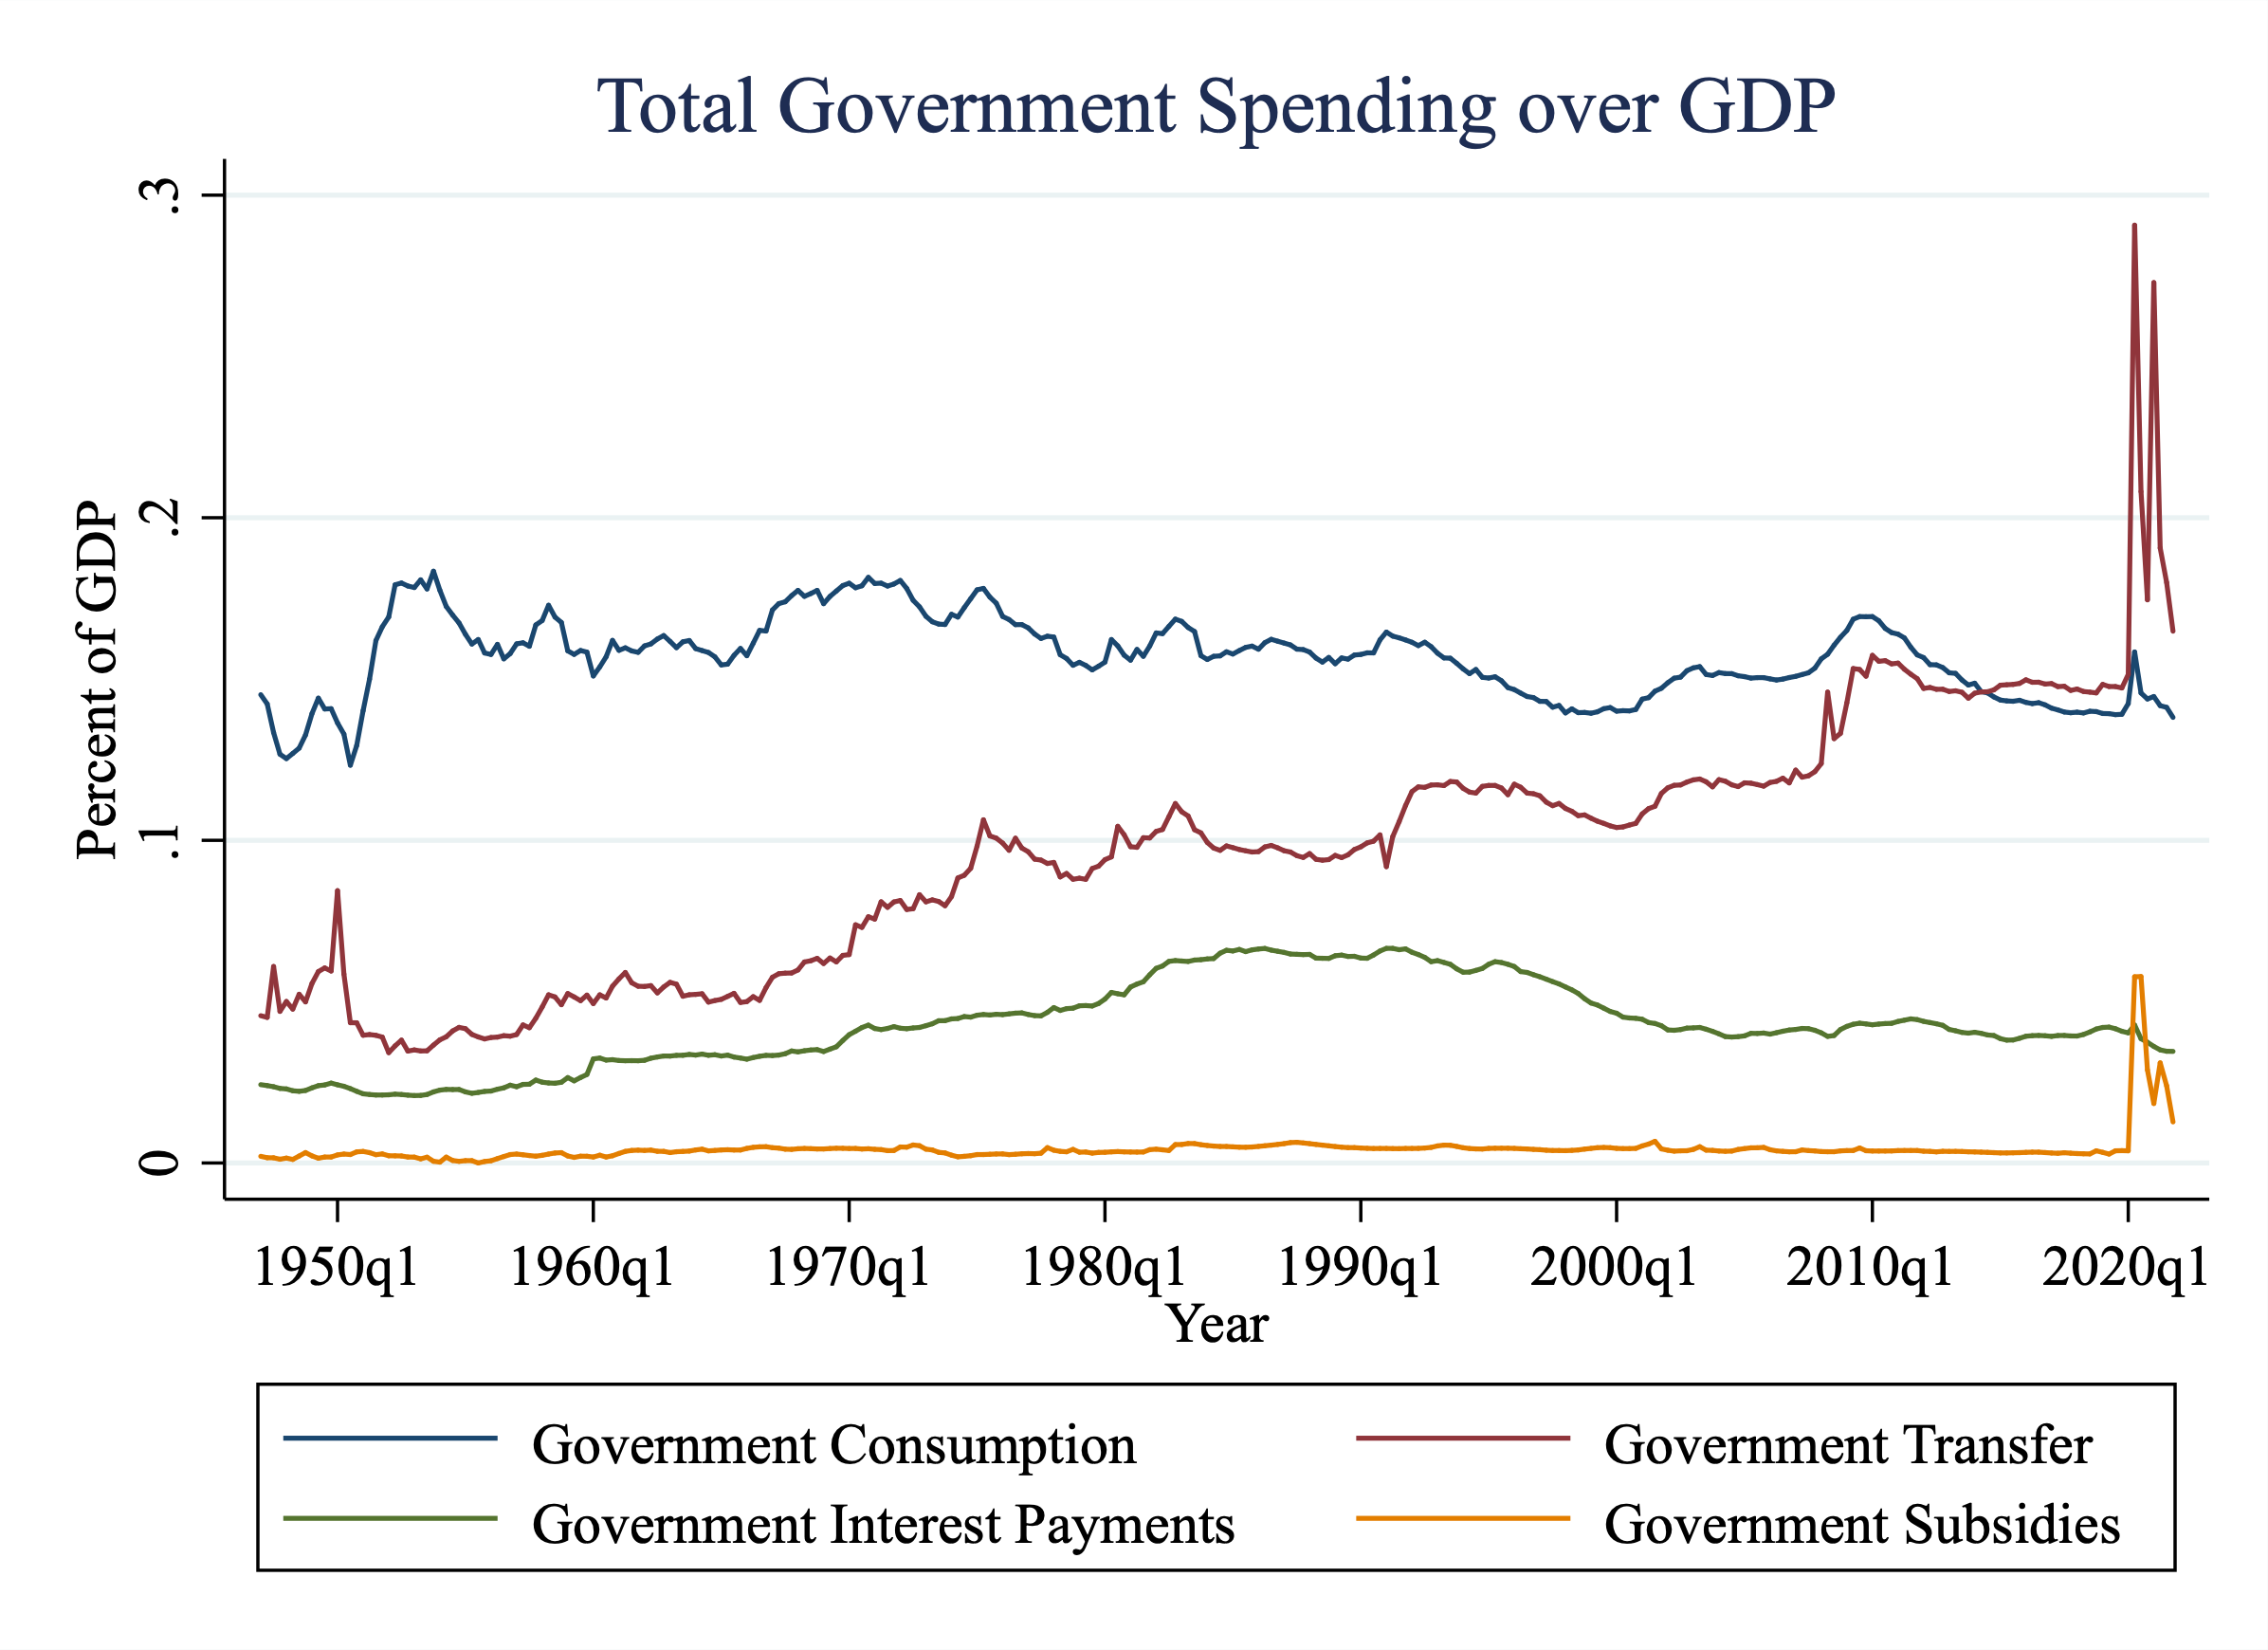
\includegraphics[scale=0.2]{Figures/GoverY_3.png}
\end{figure}
Rise in government spending comes from transfers, rather than consumption or subsidies or interest payments
\end{frame}


\begin{frame}
\frametitle[alignment=center]{$G\neq T$!}
\begin{figure}
\centering
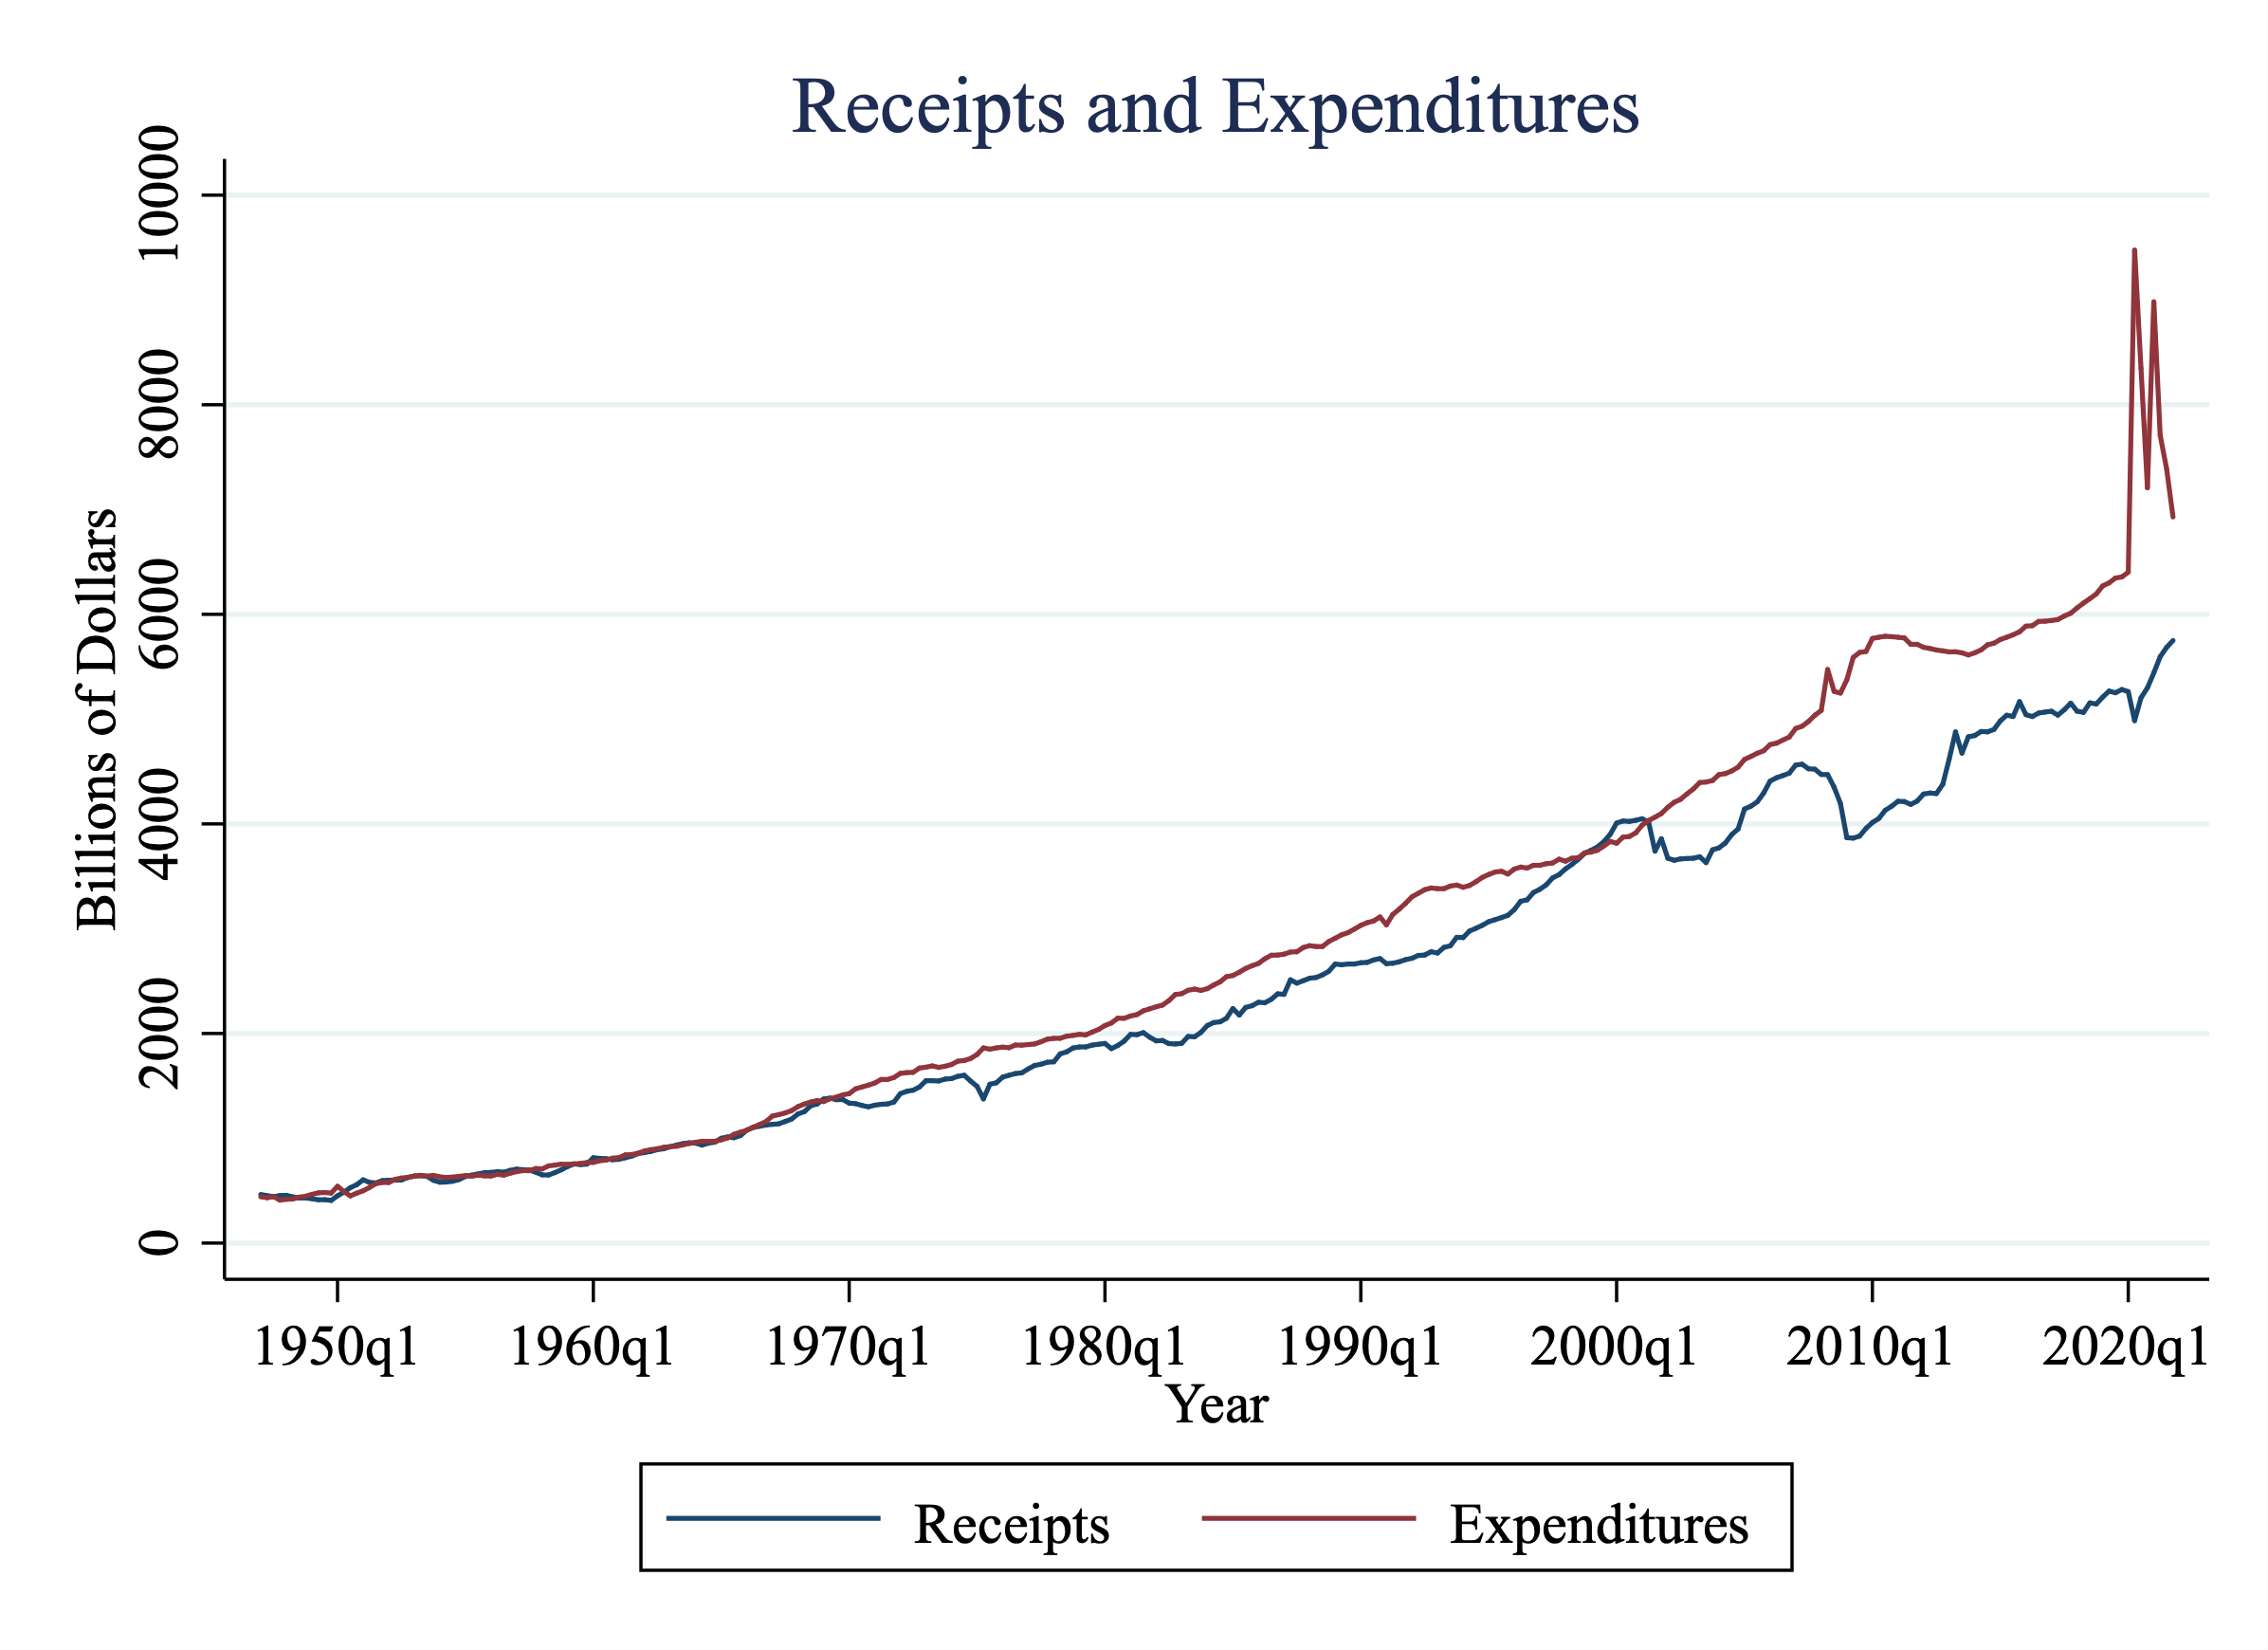
\includegraphics[scale=0.2]{Figures/GoverY_4.png}
\end{figure}
Also note that our $G=T$ assumption is wrong
\end{frame}

\begin{frame}
\frametitle[alignment=center]{Same thing, but over GDP}
\begin{figure}
\centering
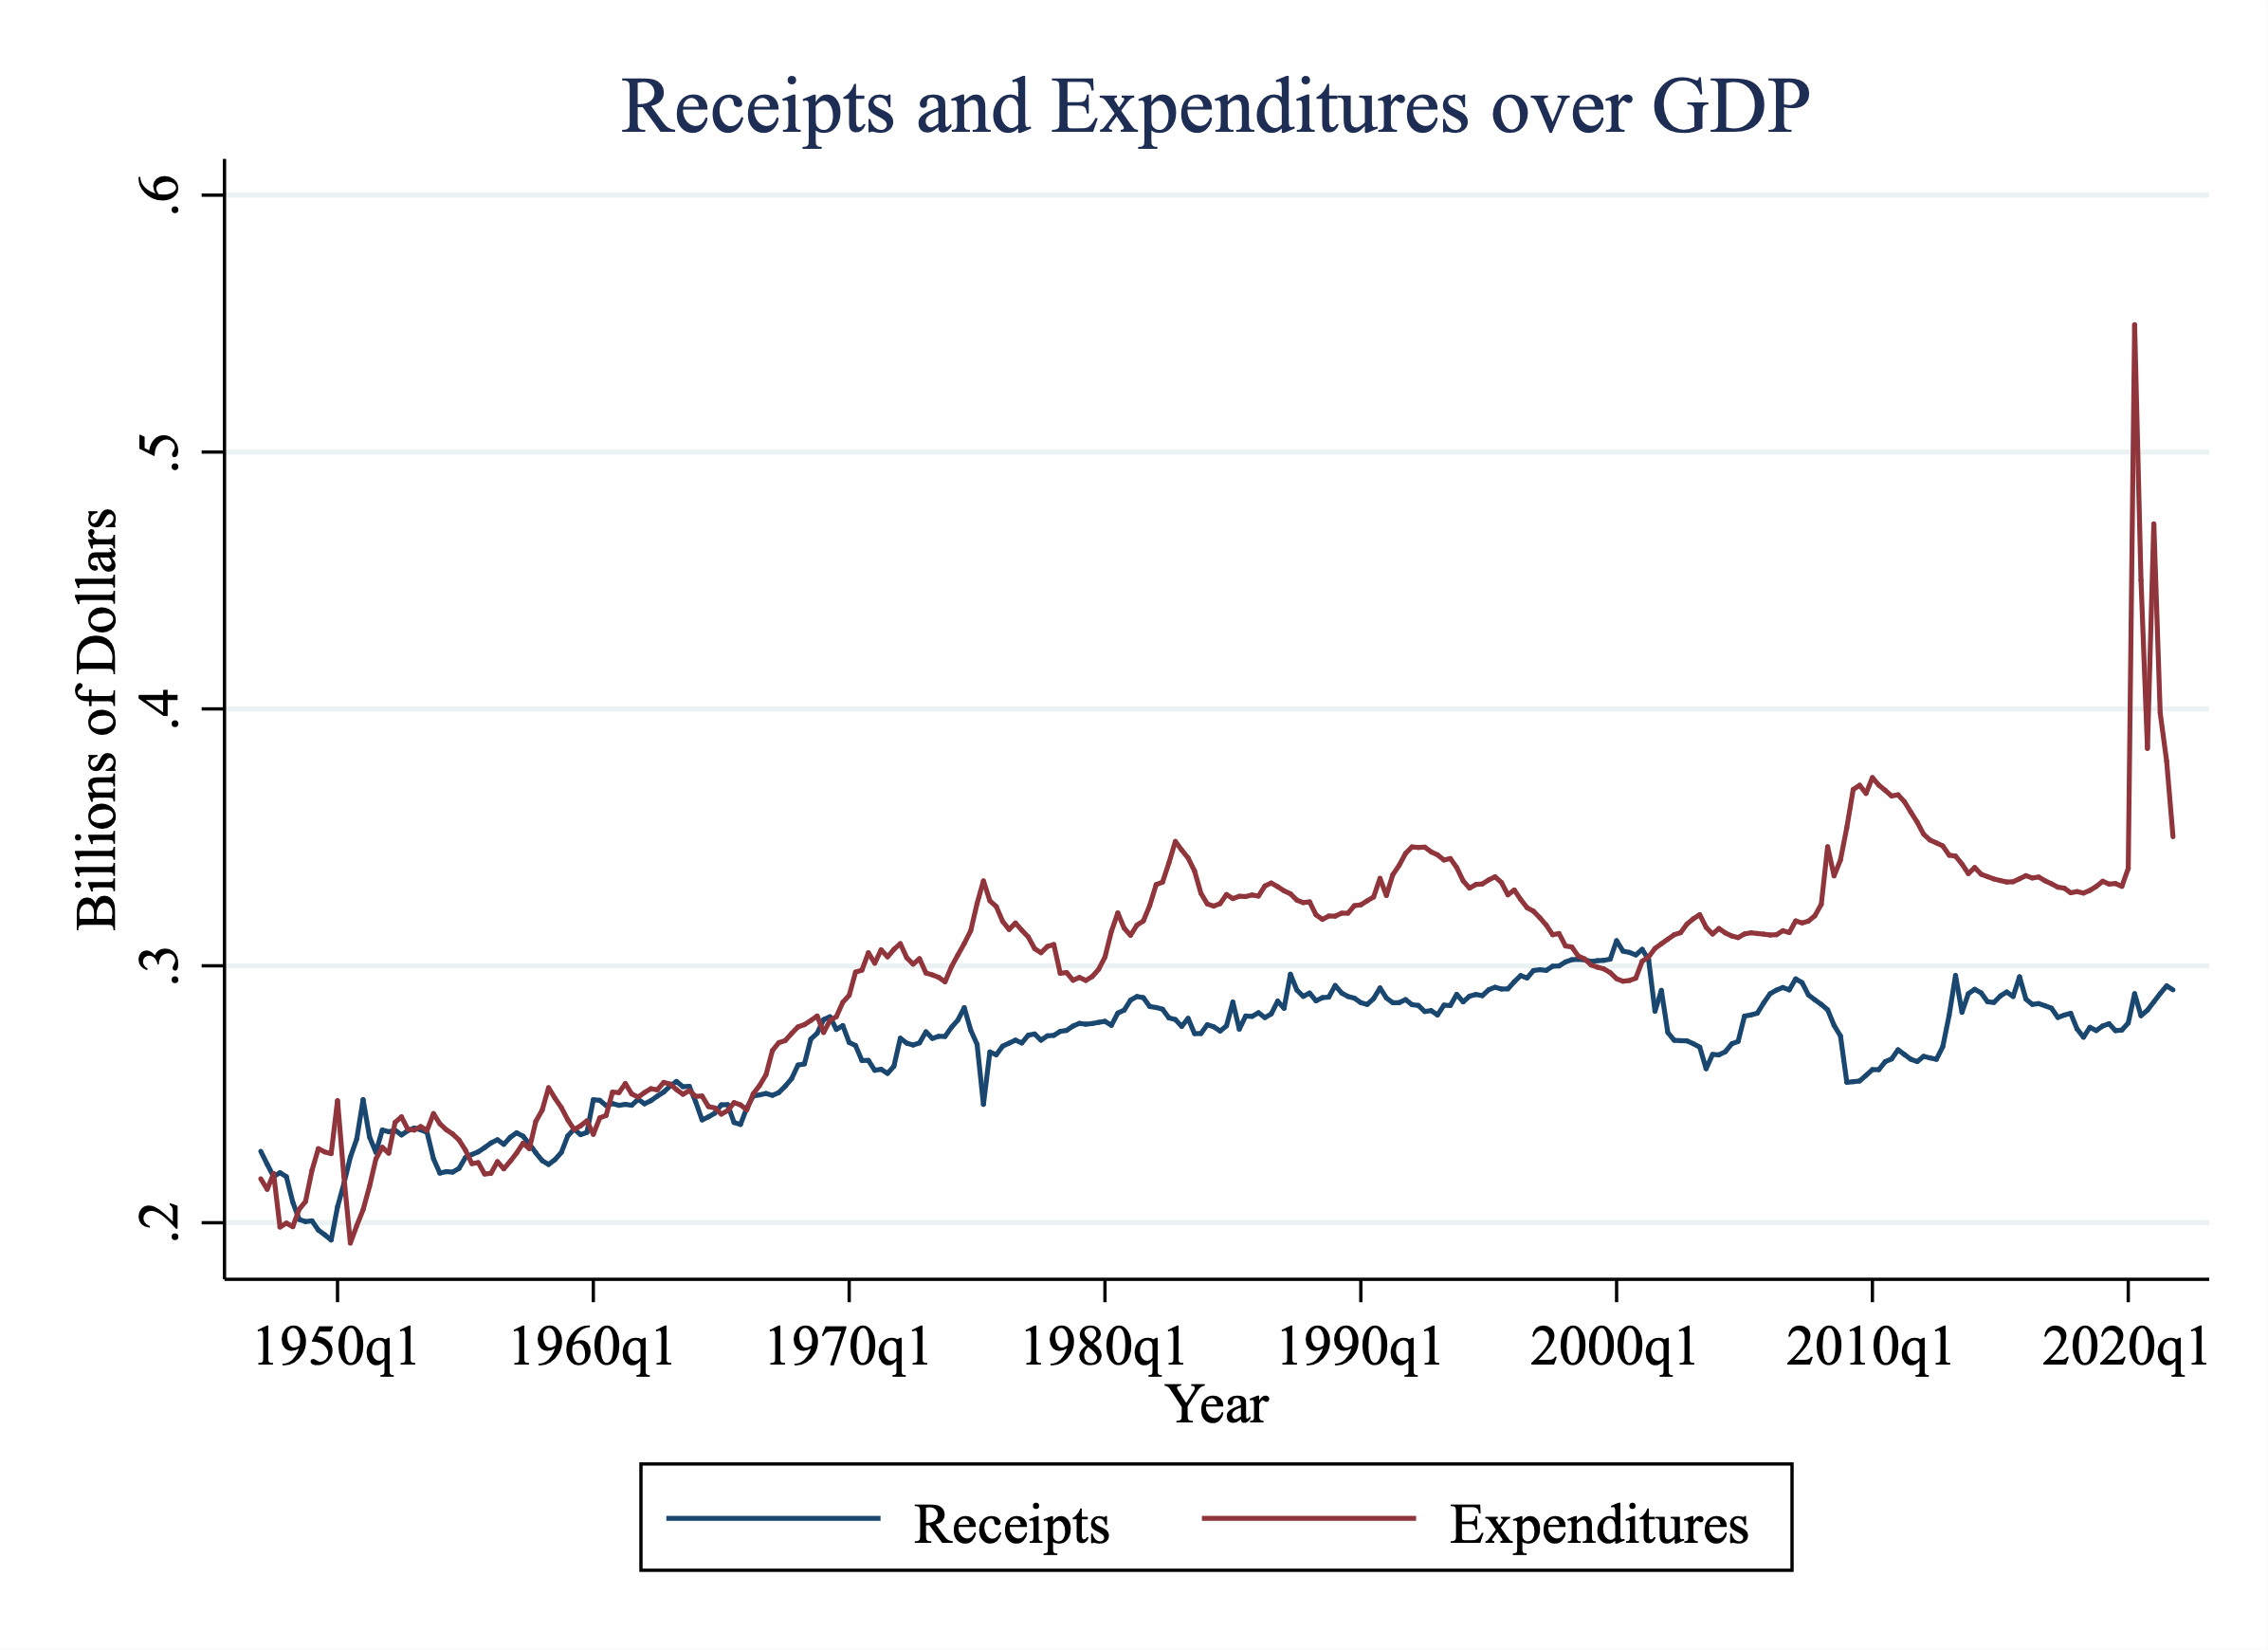
\includegraphics[scale=0.2]{Figures/GoverY_5.png}
\end{figure}
\end{frame}


\begin{frame}
\frametitle[alignment=center]{Taxes}
\begin{itemize}
\item So far, the household budget constraint has been $C=wn+\pi-T$
\bigskip
\item But $T$ really depends on $wn$: make more, pay more
\bigskip
\item This distorts behavior (income and substitution effects, where the other was just income)
\bigskip
\item Instead, we'll change the budget constraint so that:
$$C=w(1-\tau)(h-\ell)+\pi$$
\item Where, as a reminder, $C$ is consumption, $w$ is wages, $\tau$ is the (new!) ``proportional tax rate" $h$ is how much free time you have, $\ell$ is leisure, and $\pi$ is profits
\bigskip
\item We'll simplify the production function so that it's linear:
$$Y=zN^d$$
\end{itemize}
\end{frame}

\begin{frame}
\frametitle[alignment=center]{Labor Demand}
\begin{itemize}
\item Profit of the firm:
$$\pi=Y-wN^d=zN^d-wN^d$$
\item FOC of the firm: $\frac{\partial \pi}{\partial N^d}=0$:
$$w=z$$
\item Note that it does not depend on labor!  Horizontal ``perfectly elastic" demand curve
\end{itemize}
\end{frame}

\begin{frame}
\frametitle[alignment=center]{PPF with a Linear Production Function}
\begin{figure}
\centering
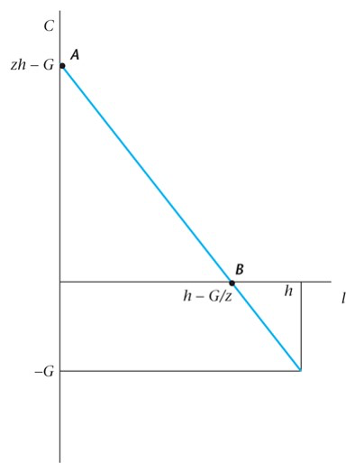
\includegraphics[scale=0.5]{Figures/W_Fig_5pt14.png}
\end{figure}
\end{frame}


\begin{frame}
\frametitle[alignment=center]{Labor Demand in Simplified Model}
\begin{figure}
\centering
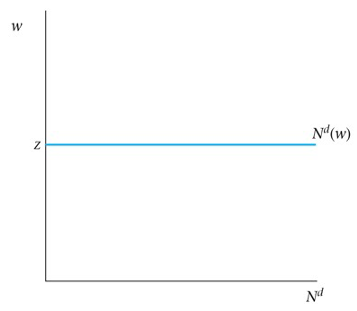
\includegraphics[scale=0.5]{Figures/W_Fig_5pt15.png}
\end{figure}
\end{frame}


\begin{frame}
\frametitle[alignment=center]{Shifting with a proportional tax}
\begin{itemize}
\item Now, our PPF shifts with a proportional tax on labor income
\bigskip
\item So let's compare two experiments:  one in which we graph the old, lump-sum tax, and the other in which we have a proportional tax
\end{itemize}
\end{frame}

\begin{frame}
\frametitle[alignment=center]{Labor Demand in Simplified Model}
\begin{figure}
\centering
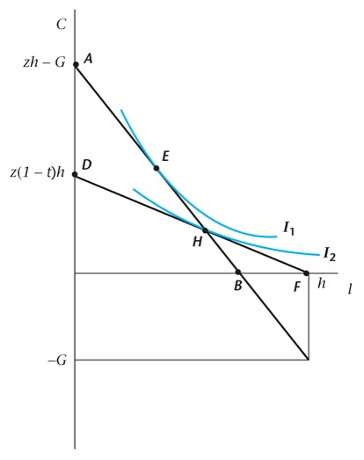
\includegraphics[scale=0.5]{Figures/W_Fig_5pt16.png}
\end{figure}
\end{frame}


\begin{frame}
\frametitle[alignment=center]{Laffer Curve}
\begin{itemize}
\item Rather than fixing $G$ and examining what happens for a lump-sum vs a distortionary tax, we could instead think about $G$ as a function of $\tau$
\bigskip
\item Revenue from a proportional tax on labor is: 
$$Rev=\tau n$$
\item But, as we saw, $n$ is a function of $\tau$!  So more clearly:
$$Rev=\tau n(\tau)$$
\item There's a tension: when $\tau\uparrow$, $n(\tau)\downarrow$
\bigskip
\item When $\tau=1$, $L(\tau)=$, so $Rev=\tau L(\tau)=0$, and when $\tau=0$, $Rev=\tau L(\tau)=0$.  But presumably $Rev>0$ for some $\tau$ in between--this is the ``Laffer Curve"
\end{itemize}
\end{frame}

\begin{frame}
\frametitle[alignment=center]{Idealized Laffer Curve}
\begin{figure}
\centering
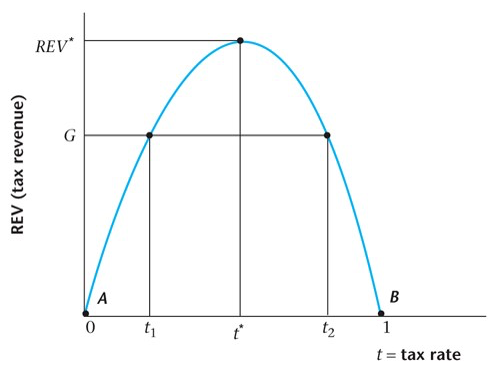
\includegraphics[scale=0.5]{Figures/W_Fig_5pt17.png}
\end{figure}
\end{frame}


\begin{frame}
\frametitle[alignment=center]{Two Equilibria}
\begin{figure}
\centering
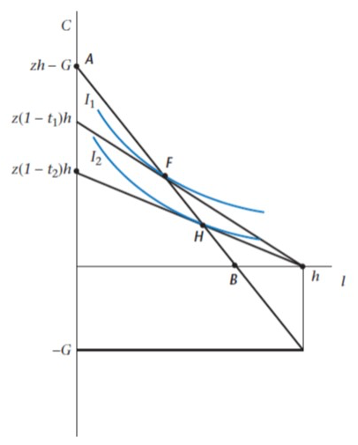
\includegraphics[scale=0.5]{Figures/W_Fig_5pt18.png}
\end{figure}
\end{frame}


\begin{frame}
\frametitle[alignment=center]{Concrete Example}
\begin{itemize}
\item Let's go back to our tax example, where we found:
$$n=\frac{1-\tau}{4}\ \ \ C=\frac{(1-\tau)^2}{4}$$
\item Then in that example ($w=1\Rightarrow Y=N^d$):
$$Rev=\tau \frac{1-\tau}{4}$$
\item Or:
$$Rev=\frac{\tau}{4}-\frac{\tau^2}{4}$$
\item There are two worlds that generate the same revenue! Let's look when $Rev=0.03$ 
\end{itemize}
\end{frame}


\begin{frame}
\frametitle[alignment=center]{Our Laffer Curve}
\begin{figure}
\centering
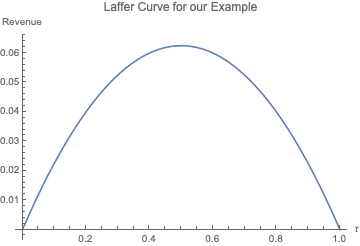
\includegraphics[scale=0.5]{Figures/Laffer.png}
\end{figure}
\end{frame}


\begin{frame}
\frametitle[alignment=center]{Concrete Example-Two Equilibria}
\begin{table}
\begin{tabular}{lccc}
\multicolumn{4}{c}{Laffer Curve Example}\\
\hline\hline
Variable & Notation & Regime 1 & Regime 2 \\
\hline
Revenue & $Rev$ & 0.03 & 0.03 \\
Tax rate & $\tau$ & 0.139 & 0.861 \\
Labor & $n$ & 0.215 & 0.034 \\
Consumption & $C$ & 0.185 & 0.005 \\
Utility & $U$ & 0.215 & 0.035 \\
Equivalent Variation & $CV$ & $-0.1$ & $\cdot$
\end{tabular}
\end{table}
\begin{itemize}
\item Equivalent variation solves the problem, roughly $U(C_1+\delta,n_1)=U(C_2,n_2)$, e.g. how much would person in Regime 1 would have to lose (lump sum!) in order to be just as badly off as the person in Regime 2.  
\bigskip
\item The interpretation here is that a person in Regime 1 would be willing to give up 45\% of their consumption just to stay in that regime!
\end{itemize}
\end{frame}



\begin{frame}
\frametitle[alignment=center]{How Large should Government Be?}
\begin{itemize}
\item Up until now, we've taken the size of government as given
\bigskip
\item But obviously that's someone's choice as well!
\bigskip
\item Recall that: $Y=C+T$
\bigskip
\item Let's say that the government takes 1 unit of private consumption good and turns it into $q$ units of public goods, so that:
$$C=Y-\frac{G}{q}$$
\item q is some measure of government efficiency. 
\bigskip
\item Then we can write out the ``societal" PPF of C vs G
\end{itemize}
\end{frame}

\begin{frame}
\frametitle[alignment=center]{Optimal Choice of Government Spending}
\begin{figure}
\centering
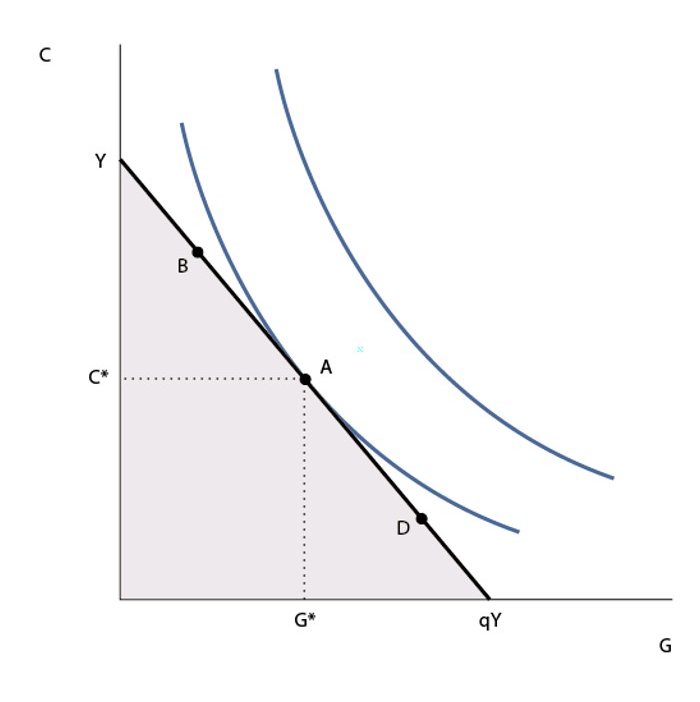
\includegraphics[scale=0.5]{Figures/W_Fig_5pt19.png}
\end{figure}
How do shifts in $z$, $q$ affect our decision?
\end{frame}

\begin{frame}
\frametitle[alignment=center]{Optimal Choice of Government Spending}
\begin{figure}
\centering
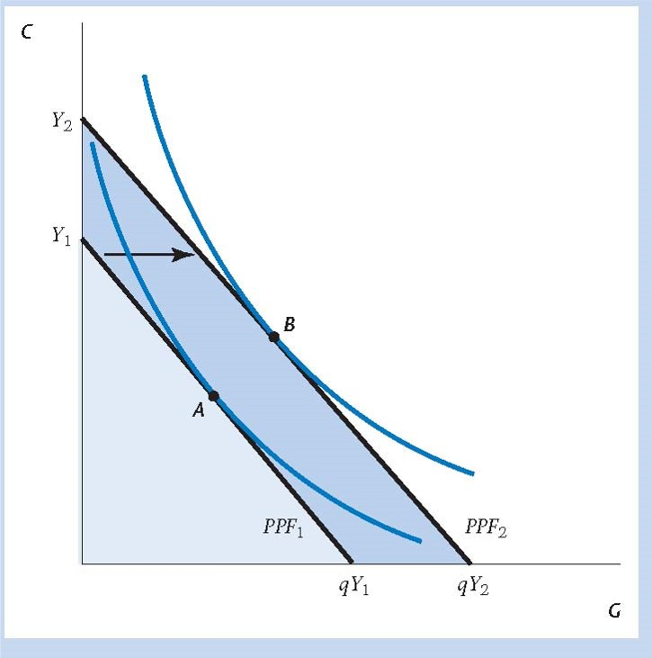
\includegraphics[scale=0.5]{Figures/W_Fig_5pt20.png}
\end{figure}
An increase in $z$ clearly suggests an increase in $C$ and $G$ (this assumes $G$ is normal)
\end{frame}


\begin{frame}
\frametitle[alignment=center]{Optimal Choice of Government Spending}
\begin{figure}
\centering
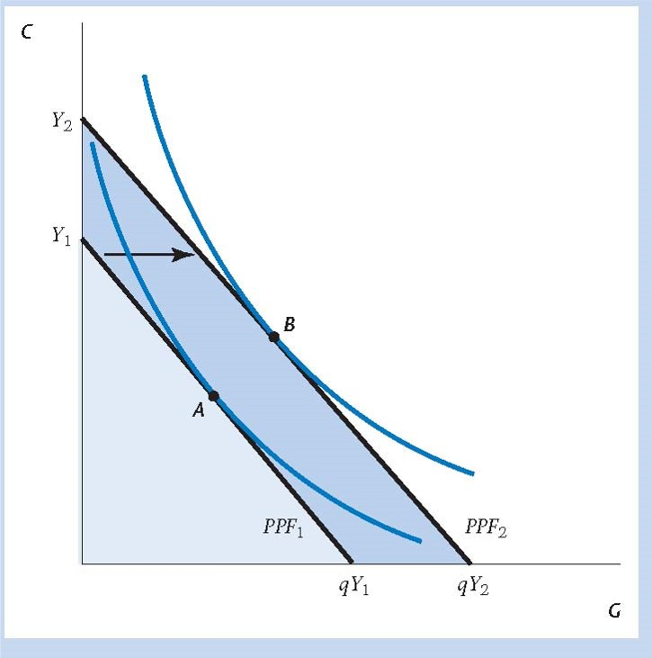
\includegraphics[scale=0.5]{Figures/W_Fig_5pt20.png}
\end{figure}
An increase in $q$ suggests $G$ must increase, what happens to $C$ is ambiguous (income and substitution effects)
\begin{itemize}
\item Presents interesting dilemma for a small-government type:  do I want government to be efficient or not?  
\end{itemize}
\end{frame}

\begin{frame}
\frametitle[alignment=center]{Conclusions}
\begin{itemize}
\item This was a big chapter!
\bigskip
\item Now we can take consumer \& firm behavior and \textbf{start} thinking about various choices, such as:
\begin{itemize}
\item When the government increases flat tax $T$, should I work more or less?  Consume more or less?
\bigskip
\item When the government increases proportional tax $\tau$, should I work more or less?  Consume more or less?
\bigskip
\item When  TFP  $z$ increases, what happens to $C$, $n$, etc.
\bigskip
\item What is the optimal size of government?  
\end{itemize}
\item We also saw our first simple numerical models of consumer behavior, cousins to what modern macroeconomists really use
\bigskip
\item Next we'll turn to search \& unemployment:  frictions
\end{itemize}
\end{frame}




\end{document}